\documentclass{bestbeamer}

\title[Models causals estructurals i resultats potencials]{Models causals estructurals\\i resultats potencials}
\subtitle{El ciment del món}
\author{Mario \textsc{Vilar}}
\advisors{Dr.~Jordi \textsc{Vitrià}}{Dr.~Josep \textsc{Vives}}
\institute{Treball de Final de Grau\\Universitat de Barcelona}
\date{2 de juliol de 2026}
\bestrepository{https://github.com/mariovilar/TFG}

\hypersetup{
  pdftitle={Models causals estructurals i resultats potencials},
  pdfauthor={Mario Vilar},
  pdfsubject={Defensa del Treball de Final de Grau},
  hidelinks,
  linkcolor=bestLink,
  urlcolor=bestLink
}
\addbibresource{res/bibl.bib}

\tikzset{
  causal node/.style={
    circle,
    draw=bestDiagramInk,
    fill=white,
    minimum size=7.5mm,
    inner sep=1pt,
    font=\small
  },
  causal arrow/.style={-{Stealth[length=2.2mm]},semithick,bestDiagramInk},
  confounding/.style={
    {Stealth[length=2.1mm]}-{Stealth[length=2.1mm]},
    dashed,
    semithick,
    bestDiagramMuted
  },
  flow box/.style={
    draw=bestDiagramMid,
    fill=bestDiagramLight,
    rounded corners=1pt,
    minimum height=9mm,
    align=center,
    inner xsep=5pt,
    font=\small
  }
}

\begin{document}

\part{Defensa}

\begin{frame}[plain]
  \titlepage
\end{frame}

\begin{frame}{Índex}
  \tableofcontents[part=1,hideallsubsections]
\end{frame}

\section{Introducció}
\subsection{Causalitat}
\begin{frame}{Què és la causalitat}
\begin{figure}
\centering
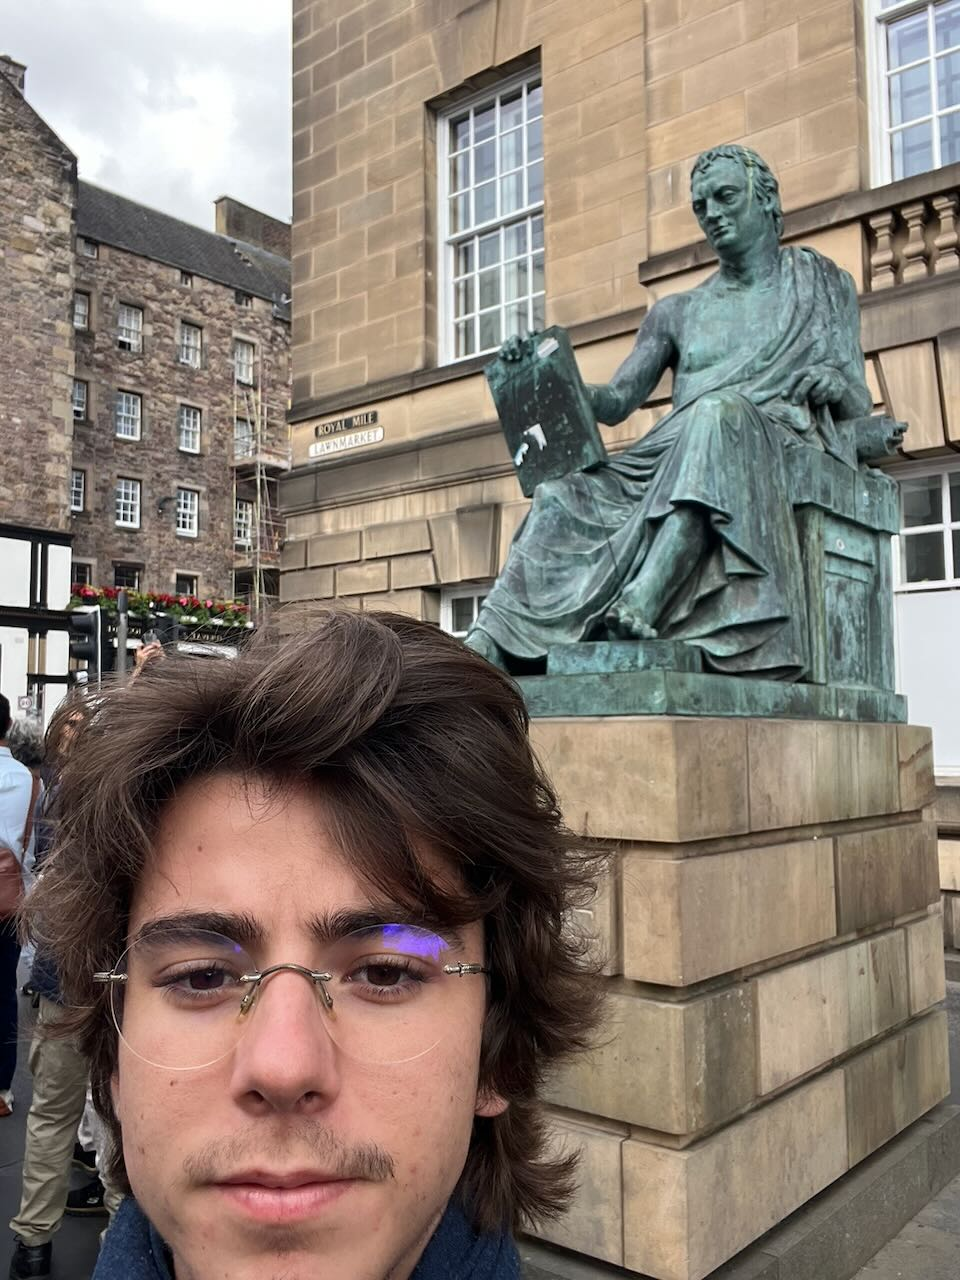
\includegraphics[width=0.3\textwidth]{res/hume.jpeg}
% \caption{Estàtua de Hume a Edimburg (Escòcia) i un servidor.}
\label{fig:hume}
\end{figure}
\end{frame}

\begin{comment}
\begin{minipage}[t]{.64\textwidth}
\begin{itemize}
  \item Regularisme \cite{hume2000treatise}
  \item Contrafactuals \cite{Mill1843,lewis1973comparative,lewis1981counterfactuals}
  \item Diagrames de camins i coeficients de camí \cite{wright1921correlation}
  \item Intervencions \cite{woodward2003making,pearl2009causality}
  \item Mecanicisme, pluralisme, poders causals...
\end{itemize}
\end{minipage}
\end{comment}

\begin{frame}{Què no és la causalitat}
\begin{center}
\includesvg[
  width=.86\textwidth,
  height=.68\textheight,
  keepaspectratio,
  inkscapelatex=false
]{res/rainfall}
\bestsource{Dades i exemple adaptats de \cite{vigen_spurious}.}
\end{center}
\end{frame}

\subsection{Jerarquia causal}
\begin{comment}
\begin{frame}{La jerarquia causal de Pearl I \texorpdfstring{\cite{pearl2018book}}{}}
  \hypertarget{frame:pearl-hierarchy-i}{}
  \centering
  \begin{columns}[T,onlytextwidth]
    \begin{column}{.49\textwidth}
      \centering
      {\bfseries Món observacional}

      \vspace{2mm}
      \begin{tikzpicture}[
        scale=.82,
        transform shape,
        node distance=8mm and 8mm,
        pearl node/.style={
          circle,
          draw=bestDiagramInk,
          fill=white,
          minimum size=7.6mm,
          inner sep=0pt,
          font=\scriptsize\bfseries
        },
        pearl label/.style={font=\scriptsize,align=center,bestDiagramInk},
        pearl arrow/.style={causal arrow,bestDiagramInk}
      ]
        \node[pearl node] (tribunal) {J};
        \node[pearl label,above=1mm of tribunal] {Jutge};
        \node[pearl node,below=of tribunal] (capita) {K};
        \node[pearl label,left=1mm of capita] {Capità};
        \node[pearl node,below left=of capita] (a) {A};
        \node[pearl label,left=1mm of a] {Tirador A};
        \node[pearl node,below right=of capita] (b) {B};
        \node[pearl label,right=1mm of b] {Tirador B};
        \node[pearl node,below=15mm of capita] (mort) {M};
        \node[pearl label,below=1mm of mort] {Mort};

        \draw[pearl arrow] (tribunal) -- (capita);
        \draw[pearl arrow] (capita) -- (a);
        \draw[pearl arrow] (capita) -- (b);
        \draw[pearl arrow] (a) -- (mort);
        \draw[pearl arrow] (b) -- (mort);
      \end{tikzpicture}
    \end{column}
    \begin{column}{.49\textwidth}
      \centering
      {\bfseries Món intervingut}

      \vspace{1mm}
      \begin{tikzpicture}[
        scale=.82,
        transform shape,
        node distance=8mm and 8mm,
        pearl node/.style={
          circle,
          draw=bestDiagramInk,
          fill=white,
          minimum size=7.6mm,
          inner sep=0pt,
          font=\scriptsize\bfseries
        },
        intervened node/.style={
          pearl node,
          draw=bestAirforce700,
          fill=bestAirforce100,
          line width=.6pt
        },
        pearl label/.style={font=\scriptsize,align=center,bestDiagramInk},
        pearl arrow/.style={causal arrow,bestDiagramInk},
        cut arrow/.style={pearl arrow,dashed,bestDiagramMuted}
      ]
        \node[pearl node] (tribunal) {J};
        \node[pearl label,above=1mm of tribunal] {Jutge};
        \node[pearl node,below=of tribunal] (capita) {K};
        \node[pearl label,left=1mm of capita] {Capità};
        \node[intervened node,below left=of capita] (a) {A};
        \node[pearl label,left=1mm of a] {Tirador A};
        \node[pearl node,below right=of capita] (b) {B};
        \node[pearl label,right=1mm of b] {Tirador B};
        \node[pearl node,below=15mm of capita] (mort) {M};
        \node[pearl label,below=1mm of mort] {Mort};

        \draw[pearl arrow] (tribunal) -- (capita);
        \draw[cut arrow] (capita) -- (a);
        \draw[pearl arrow] (capita) -- (b);
        \draw[pearl arrow] (a) -- (mort);
        \draw[pearl arrow] (b) -- (mort);

        \draw[bestAirforce700,line width=.8pt]
          ($(capita)!0.45!(a)+(-.08,.08)$) -- ($(capita)!0.45!(a)+(.08,-.08)$);
        \draw[bestAirforce700,line width=.8pt]
          ($(capita)!0.45!(a)+(.08,.08)$) -- ($(capita)!0.45!(a)+(-.08,-.08)$);
      \end{tikzpicture}
    \end{column}
  \end{columns}

  \vspace{-1mm}
  \hfill\bestlinkbutton{frame:do-operator}{\texttt{do()}}
\end{frame}
\end{comment}

\begin{frame}{La jerarquia causal de Pearl}
  \centering
  \begin{tikzpicture}[x=1cm,y=1cm]
    \fill[bestDiagramLight] (0,0) rectangle (4.0,1.05);
    \fill[bestAirforce200] (1.25,1.05) rectangle (5.25,2.10);
    \fill[bestDiagramMid] (2.50,2.10) rectangle (6.50,3.15);

    \node[anchor=west,font=\bfseries] at (.25,.72) {$\mathcal L_1$ Associació};
    \node[anchor=west,font=\small] at (.25,.30) {Què passa si observo $X$?};

    \node[anchor=west,font=\bfseries] at (1.50,1.77) {$\mathcal L_2$ Intervenció};
    \node[anchor=west,font=\small] at (1.50,1.35) {Què passa si faig $X$?};

    \node[anchor=west,font=\bfseries] at (2.75,2.82) {$\mathcal L_3$ Contrafactual};
    \node[anchor=west,font=\small] at (2.75,2.40) {Què hauria passat si...?};

    \draw[causal arrow,bestAirforce600] (6.85,.4) -- (6.85,2.85);
    \node[rotate=90,anchor=south,font=\scriptsize,bestDiagramMuted]
      at (7.34,1.62) {més estructura causal};
    \node[rotate=90,anchor=south,font=\scriptsize,bestDiagramMuted]
      at (7.64,1.62) {(hipòtesis, coneixement extern...)};
  \end{tikzpicture}

  \vspace{2mm}
  \begin{columns}[T,onlytextwidth]
    \begin{column}{.30\textwidth}
      \centering
      \[
        P(Y\mid X=x)
      \]
      \small Predicció i diagnòstic \\
      \textit{(observo)}
    \end{column}
    \begin{column}{.34\textwidth}
      \centering
      \[
        P(Y\mid\doop(X=x))
      \]
      \small Accions, polítiques i decisions \\
      \textit{(intervinc)}
    \end{column}
    \begin{column}{.32\textwidth}
      \centering
      \[
        P(Y_x\mid X=x',Y=y)
      \]
      \small Explicació i mons alternatius \\
      \textit{(imagino)}
    \end{column}
  \end{columns}
\end{frame}

\section{Models causals estructurals (Pearl)}
\subsection{Xarxes bayesianes}

\begin{frame}{Regla de la cadena}
\begin{itemize}
  \item Sigui $\G=(\V,\EE)$ un \textit{graf acíclic dirigit} (DAG), $\V=\{V_i\}_{i\in I}$ el conjunt de variables, $I=\{1,\dotsc,n\}$ el conjunt d'índexs i $\EE\subseteq \V\times \V$ el conjunt d'arestes del graf. 
  \item Sigui $(\Omega,\mathcal{F},\mathbb{P})$ un espai de probabilitat, on $\Omega$ és l'espai mostral i $\mathbb{P}:\mathcal{F}\longrightarrow[0,1]$ és una mesura de probabilitat sobre $(\Omega,\mathcal{F})$ tal que $P:=P(\V)$ és la llei conjunta de $\V$.
  \item $(\mathcal{X}_i,\mathcal{B}(\mathcal{X}_i))_{i\in I}$ espais de Borel estàndard, tals que $(\mathcal{X},\mathcal{B}(\mathcal{X}))=(\prod_{i=1}^n\mathcal{X}_i,\bigotimes_{i=1}^n\mathcal{B}(\mathcal{X}_i))$. Escrivim $\vvv=(v_i)_{i\in I}\in\mathcal{X}$. $\operatorname{Pa}_i^\mathcal{G}=\{V_j\in\V \mid V_j\to V_i\in\EE\}\subsetneq\V$ són els \textit{pares gràfics}.
\end{itemize}
\begin{definition}[Xarxa bayesiana]
Una \textit{xarxa bayesiana} és un parell $(\G,P)$ on $P$ factoritza sobre $\G$. Diem que $P$ factoritza sobre $\G$ si $p(v_1,\dotsc,v_n)=\prod_{i=1}^n p(v_i\mid v_1,\dotsc,v_{i-1})=\prod_{i=1}^n p(v_i\mid \operatorname{pa}_i^{\G})$.
\end{definition}
\end{frame}

\subsection{Configuracions gràfiques}
\begin{frame}{\texorpdfstring{$d$-separació}{d-separació}, cadenes, bifurcacions i col·lisionadors}
\begin{definition}[{\cite[Def.~1.2.3]{pearl2009causality}}]\label{def:dseparacio}
Diem que $\XX,\YY\subseteq\V$ (amb $\XX\cap\YY=\emptyset$) estan $d$-separats per $\ZZ$ (amb $\XX\cap\ZZ=\YY\cap\ZZ=\emptyset$) si \textit{cada} camí entre les variables de $\XX$ i les variables de $\YY$ està blocat per $\ZZ$.
\begin{equation*}
\XX\perp_\G \YY\mid \ZZ.
\end{equation*}
\end{definition}
\begin{figure}
  \centering
  \begin{tikzpicture}[
    cond node/.style={
      causal node,
      draw=bestDiagramAccentA,
      fill=bestDiagramLight,
      double=bestDiagramAccentA,
      double distance=.8pt
    },
    blocked path/.style={
      bestDiagramAccentA,
      line width=.8pt,
      line cap=round
    },
    diagram label/.style={font=\scriptsize,bestDiagramMuted}
  ]
    \begin{scope}[xshift=-4.15cm]
      \node[causal node] (cx) at (-1.32,0) {$X$};
      \node[cond node] (cz) at (0,0) {$Z$};
      \node[causal node] (cy) at (1.32,0) {$Y$};
      \draw[causal arrow] (cx) -- (cz);
      \draw[causal arrow] (cz) -- (cy);
      \draw[blocked path] ($(cz)+(-.42,.42)$) -- ($(cz)+(.42,-.42)$);
      \draw[blocked path] ($(cz)+(-.42,-.42)$) -- ($(cz)+(.42,.42)$);
      \node[diagram label,below=5mm of cz] {cadena};
    \end{scope}

    \begin{scope}
      \node[causal node] (fx) at (-1.32,0) {$X$};
      \node[cond node] (fz) at (0,0) {$Z$};
      \node[causal node] (fy) at (1.32,0) {$Y$};
      \draw[causal arrow] (fz) -- (fx);
      \draw[causal arrow] (fz) -- (fy);
      \draw[blocked path] ($(fz)+(-.42,.42)$) -- ($(fz)+(.42,-.42)$);
      \draw[blocked path] ($(fz)+(-.42,-.42)$) -- ($(fz)+(.42,.42)$);
      \node[diagram label,below=5mm of fz] {bifurcació};
    \end{scope}

    \begin{scope}[xshift=4.15cm]
      \node[causal node] (kx) at (-1.32,0) {$X$};
      \node[causal node] (kz) at (0,0) {$Z$};
      \node[causal node] (ky) at (1.32,0) {$Y$};
      \draw[causal arrow] (kx) -- (kz);
      \draw[causal arrow] (ky) -- (kz);
      \draw[blocked path] ($(kz)+(-.42,.42)$) -- ($(kz)+(.42,-.42)$);
      \draw[blocked path] ($(kz)+(-.42,-.42)$) -- ($(kz)+(.42,.42)$);
      \node[diagram label,below=5mm of kz] {col·lisionador};
    \end{scope}
  \end{tikzpicture}
  \bestsource{\cite[Def.~1.2.3]{pearl2009causality}.}
  \label{fig:cincvariables}
\end{figure}
\end{frame}

\subsection{SCMs}
\begin{frame}{Models causals estructurals}\label{frame:SCMs}
\begin{definition}[{\cite[Def.~27.1]{bareinboim2022}; \cite[Sec.~1.4.1]{pearl2009causality}}]\label{def:scm}
Definim un SCM (\emph{Structural Causal Model}) com $\mathcal{M} = (\U,\V,\mathcal{F},P(\U))$, on:
\begin{itemize}
    \item $\U$ és el conjunt de variables aleatòries \emph{exògenes}.
    \item $\V$ és el conjunt de variables \emph{endògenes}. 
    \item Per a cada $V_i\in\V$, denotem per $\mathbf{U}_i^c\subseteq\U$ el conjunt de factors exògens associats a $V_i$ i per $\operatorname{Pa}_i^\M\subseteq\V\setminus\{V_i\}$ els \textit{pares estructurals}.
    \item $\mathcal{F}=\{f_i\}_{i\in I}$ és un conjunt de \textit{funcions estructurals} $f_i(\operatorname{pa}_i^\mathcal{M},\mathbf{u}_i^c)$ amb $i\in I$.
    \item $P(\U)$ és la llei del vector aleatori $\UU:(\Omega,\mathcal F)\longrightarrow(\mathfrak U,\mathcal B(\mathfrak U))$.
\end{itemize}
\end{definition}
\vfill
\hfill\bestlinkbutton{frame:SCM2}{Funcions estructurals}
\end{frame}

\begin{frame}{El tabac i el càncer de pulmó}
  \begin{columns}[T,onlytextwidth]
    \begin{column}{.7\textwidth}
      \begin{enumerate}
        \item El tabac causa càncer de pulmó \cite{doll1950smoking}: $T\to C$.
        \item Un factor genètic inobservable $G$ provoca ganes de fumar i càncer de pulmó \cite{fisher1958cigarettes}: $T\leftrightarrow C$ ($T\leftarrow G\to C$).
      \end{enumerate}
      \begin{example}[\textit{Bow}]
      El model causal $\M=(\U,\V,\F,P(\U))$ és semi-Markovià, on $\U=\{G,U_T,U_C\}$, $\V=\{T,C\}$ i $\mathcal F=\{f_T,f_C\}$. $P(\U)=P(G)\cdot P(U_T)\cdot P(U_C)$, $\mathbf{U}_T^c=\{G,U_T\}$ i $\mathbf{U}_C^c=\{G,U_C\}$.
      \begin{equation*}
      T := f_T(\mathbf{U}_T^c),\quad C := f_C(T,\mathbf{U}_C^c).
      \end{equation*}
      Hem usat que:
      \begin{equation*}
      \operatorname{Pa}_T^\M=\emptyset, \quad \operatorname{Pa}_C^\M=\{T\}.
      \end{equation*}
      \end{example}
    \end{column}
    \begin{column}{.27\textwidth}
    \begin{figure}[H]
      \centering
      \begin{tikzpicture}[
        node distance=8mm and 6mm,
        smoke node/.style={
          circle,
          draw=bestDiagramInk,
          fill=white,
          minimum size=8.5mm,
          inner sep=0pt,
          align=center,
          font=\small
        },
        latent noise/.style={
          smoke node,
          draw=bestDiagramMuted,
          dashed
        },
        latent smoke/.style={
          smoke node,
          draw=bestDiagramMuted,
          fill=bestDiagramLight,
          dashed
        },
        smoke arrow/.style={-{Stealth[length=2.1mm]},semithick,bestDiagramInk},
        latent arrow/.style={smoke arrow,dashed,bestDiagramMuted}
      ]
        \node[latent smoke] (g) {$G$};
        \node[latent noise,below left=6mm and 4mm of g] (ut) {$U_T$};
        \node[latent noise,below right=6mm and 4mm of g] (uc) {$U_C$};
        \node[smoke node,below=16mm of ut] (t) {$T$};
        \node[smoke node,below=16mm of uc] (c) {$C$};

        \draw[smoke arrow] (t) -- (c);
        \draw[latent arrow] (g) -- (t);
        \draw[latent arrow] (g) -- (c);
        \draw[latent arrow] (ut) -- (t);
        \draw[latent arrow] (uc) -- (c);
      \end{tikzpicture}
      \bestsource{\cite{pearl2009causality}. Graf $\G_\M^+$.}
      \label{fig:cancer}
    \end{figure}
    \end{column}
  \end{columns}
\end{frame}

\section{Identificació}
\subsection{Intervencions}

\begin{frame}{Operador \texorpdfstring{\texttt{do()}}{do()} \texorpdfstring{\cite{pearl2018book}}{}}\hypertarget{frame:do-operator}{}
\small
Posem $\mathcal{P}_* = \left\{ P(\V\mid \doop(\XX=\xx)) \mid \XX \subseteq \V \right\}$. El submodel intervingut per $\doop(\xx)$ és $\M_\xx=(\U,\V,\mathcal{F}_\xx,P(\U))$, on $\mathcal{F}_\xx$ s'obté substituint, per a cada $V_i\in\XX$, l'equació estructural $V_i:=f_i(\operatorname{pa}_i^\M,\mathbf u_i^c)$ per $V_i:=x_i$.
\begin{columns}[T,onlytextwidth]
  \begin{column}{.49\textwidth}
  \centering
  \begin{tikzpicture}[
    scale=.82,
    transform shape,
    node distance=8mm and 8mm,
    pearl node/.style={
      circle,
      draw=bestDiagramInk,
      fill=white,
      minimum size=7.6mm,
      inner sep=0pt,
      font=\scriptsize\bfseries
    },
    pearl label/.style={font=\scriptsize,align=center,bestDiagramInk},
    pearl arrow/.style={causal arrow,bestDiagramInk}
  ]
    \node[pearl node] (tribunal) {J};
    \node[pearl label,above=1mm of tribunal] {Jutge};
    \node[pearl node,below=of tribunal] (capita) {K};
    \node[pearl label,left=1mm of capita] {Capità};
    \node[pearl node,below left=of capita] (a) {A};
    \node[pearl label,left=1mm of a] {Tirador A};
    \node[pearl node,below right=of capita] (b) {B};
    \node[pearl label,right=1mm of b] {Tirador B};
    \node[pearl node,below=15mm of capita] (mort) {M};
    \node[pearl label,below=1mm of mort] {Mort};

    \draw[pearl arrow] (tribunal) -- (capita);
    \draw[pearl arrow] (capita) -- (a);
    \draw[pearl arrow] (capita) -- (b);
    \draw[pearl arrow] (a) -- (mort);
    \draw[pearl arrow] (b) -- (mort);
  \end{tikzpicture}
  \end{column}
  \begin{column}{.49\textwidth}
  \centering
  \begin{tikzpicture}[
    scale=.82,
    transform shape,
    node distance=8mm and 8mm,
    pearl node/.style={
      circle,
      draw=bestDiagramInk,
      fill=white,
      minimum size=7.6mm,
      inner sep=0pt,
      font=\scriptsize\bfseries
    },
    intervened node/.style={
      pearl node,
      draw=bestAirforce700,
      fill=bestAirforce100,
      line width=.6pt
    },
    pearl label/.style={font=\scriptsize,align=center,bestDiagramInk},
    pearl arrow/.style={causal arrow,bestDiagramInk},
    cut arrow/.style={pearl arrow,dashed,bestDiagramMuted}
  ]
    \node[pearl node] (tribunal) {J};
    \node[pearl label,above=1mm of tribunal] {Jutge};
    \node[pearl node,below=of tribunal] (capita) {K};
    \node[pearl label,left=1mm of capita] {Capità};
    \node[intervened node,below left=of capita] (a) {A};
    \node[pearl label,left=1mm of a] {Tirador A};
    \node[pearl node,below right=of capita] (b) {B};
    \node[pearl label,right=1mm of b] {Tirador B};
    \node[pearl node,below=15mm of capita] (mort) {M};
    \node[pearl label,below=1mm of mort] {Mort};

    \draw[pearl arrow] (tribunal) -- (capita);
    \draw[cut arrow] (capita) -- (a);
    \draw[pearl arrow] (capita) -- (b);
    \draw[pearl arrow] (a) -- (mort);
    \draw[pearl arrow] (b) -- (mort);

    \draw[bestAirforce700,line width=.8pt]
      ($(capita)!0.45!(a)+(-.08,.08)$) -- ($(capita)!0.45!(a)+(.08,-.08)$);
    \draw[bestAirforce700,line width=.8pt]
      ($(capita)!0.45!(a)+(.08,.08)$) -- ($(capita)!0.45!(a)+(-.08,-.08)$);
  \end{tikzpicture}
  \end{column}
\end{columns}
\vspace{-2mm}
\hfill\bestlinkbutton{frame:neymanrubin}{Neyman-Rubin}
\end{frame}

\subsection{Xarxes bayesianes causals}
\begin{frame}{CBNs Markovianes i semi-Markovianes}\label{frame:CBNesquema}
  \centering
  \begin{tikzpicture}[
    x=1cm,
    y=1cm,
    panel/.style={
      draw=bestDiagramMid,
      fill=bestAirforce100!30!white,
      rounded corners=6pt,
      line width=.45pt
    },
    panel markov/.style={
      panel,
      draw=bestDiagramAccentA,
      fill=bestAirforce100!45!white
    },
    panel semi/.style={
      panel,
      draw=bestDiagramAccentB,
      fill=bestAirforce150!45!white
    },
    node base/.style={
      circle,
      draw=bestDiagramInk,
      fill=white,
      line width=.45pt,
      minimum size=6.6mm,
      inner sep=0pt,
      font=\scriptsize\bfseries
    },
    obs node/.style={node base,draw=bestDiagramMuted,fill=white},
    markov node/.style={node base,draw=bestDiagramAccentA,fill=bestAirforce100!55!white},
    semi node/.style={node base,draw=bestDiagramAccentB,fill=bestAirforce150!55!white},
    do node/.style={
      draw=bestDiagramAccentA,
      fill=white,
      rounded corners=3pt,
      inner xsep=3pt,
      inner ysep=1.5pt,
      font=\scriptsize\bfseries,
      text=bestAirforce700
    },
    do node semi/.style={do node,draw=bestDiagramAccentB},
    arrow obs/.style={-{Stealth[length=1.8mm]},semithick,bestDiagramMuted},
    arrow causal/.style={-{Stealth[length=1.8mm]},semithick,bestDiagramInk},
    arrow do/.style={-{Stealth[length=1.8mm]},semithick,bestDiagramAccentA},
    arrow semi/.style={-{Stealth[length=1.8mm]},semithick,bestDiagramAccentB},
    bidirected/.style={{Stealth[length=1.7mm]}-{Stealth[length=1.7mm]},semithick,dashed,bestDiagramMuted},
    title/.style={font=\small\bfseries,text=bestAirforce700,align=center},
    formula/.style={font=\scriptsize,align=center,text=bestAirforce700},
    tuple/.style={font=\scriptsize,text=bestAirforce700,anchor=south east},
    cut/.style={font=\large\bfseries,text=bestAirforce700}
  ]
    \begin{scope}[on background layer]
      \node[panel,minimum width=3.25cm,minimum height=3.55cm] at (0,0) {};
      \node[panel markov,minimum width=3.25cm,minimum height=3.55cm] at (3.85,0) {};
      \node[panel semi,minimum width=4.05cm,minimum height=3.55cm] at (8.15,0) {};
    \end{scope}

    \node[title] at (0,1.42) {Xarxa bayesiana};
    \node[obs node] (oz) at (-.72,.72) {$Z$};
    \node[obs node] (ox) at (-.72,-.55) {$X$};
    \node[obs node] (oy) at (.78,-.55) {$Y$};
    \draw[arrow obs] (oz) -- (ox);
    \draw[arrow obs] (oz) -- (oy);
    \draw[arrow obs] (ox) -- (oy);
    \node[tuple] at (1.42,-1.62) {$(\G,P)$};

    \node[title] at (3.85,1.42) {CBN Markoviana};
    \node[markov node] (mz) at (3.10,.72) {$Z$};
    \node[markov node] (mx) at (3.10,-.55) {$X$};
    \node[markov node] (my) at (4.60,-.55) {$Y$};
    \node[do node] (dox) at (2.90,-1.40) {\(\doop(x)\)};
    \draw[arrow obs] (mz) -- (mx);
    \draw[arrow causal] (mz) -- (my);
    \draw[arrow causal] (mx) -- (my);
    \draw[arrow do] (dox) -- (mx);
    \node[cut] at ($(mz)!0.46!(mx)$) {\(\times\)};
    \node[tuple] at (5.27,-1.62) {$(\G,\mathcal{P}_*)$};

    \node[title] at (8.15,1.42) {CBN semi-Markoviana};
    \node[semi node] (sz) at (7.40,.72) {$Z$};
    \node[semi node] (sx) at (7.40,-.55) {$X$};
    \node[semi node] (sy) at (8.95,-.55) {$Y$};
    \node[do node semi] (doxs) at (7.15,-1.40) {\(\doop(x)\)};
    \draw[arrow obs] (sz) -- (sx);
    \draw[arrow causal] (sz) -- (sy);
    \draw[arrow causal] (sx) -- (sy);
    \draw[arrow semi] (doxs) -- (sx);
    \draw[bidirected,bend left=34] (sz) to node[
      midway,
      right=.5mm,
      font=\tiny\bfseries,
      text=bestAirforce700
    ] {\(U\)} (sy);
    \node[cut] at ($(sz)!0.46!(sx)$) {\(\times\)};
    \node[tuple] at (9.97,-1.62) {$(\G,\mathcal{P}_*)$};
  \end{tikzpicture}
  \vfill
  \hfill\bestlinkbutton{frame:CBN}{Definicions formals}
  \besttakeaway{Una xarxa bayesiana descriu associacions; una CBN actua en capa $\mathcal{L}_2$ i la versió semi-Markoviana permet representar confusió latent amb arestes bidirigides.}
\end{frame}

\subsection{Front-door}

\begin{frame}{Criteri de la porta endavant}
\begin{definition}[\textit{Front-door criterion} {\cite[Sec.~1.1.4]{parafita2023}}]\label{def:front-door}
Sigui $(\mathcal{G},\mathcal{P}_*)$ una CBN semi-Markoviana, amb $P(\V)\in\mathcal{P}_*$. Considerem $\XX,\YY,\ZZ\subseteq \V$ disjunts dos a dos. $\ZZ$ satisfà el criteri de la porta endavant respecte a $(\XX,\YY)$ si:
\begin{enumerate}
    \item $\ZZ$ bloqueja tots els camins dirigits de $\XX$ a $\YY$.
    \item Tots els \textit{back-door paths} de $\XX$ a $\ZZ$ estan bloquejats per defecte i els de $\ZZ$ a $\YY$, per $\XX$.
\end{enumerate}
\end{definition}
\begin{theorem}[\textit{Front-door adjustment} {\cite[Sec.~1.1.4, Th.~2]{parafita2023}}]\label{thm:front-door}
Si $\ZZ$ satisfà el criteri de la porta endavant, aleshores per als $p(\xx),p(\xx',\zz),p(\zz\mid\xx)>0$, tenim:
{\footnotesize\begin{equation*}
    P(\YY\mid \doop(\xx))=\E_{\ZZ \mid \xx}\left[\E_{\XX}[P(\YY \mid \XX, \ZZ)]\right]=\sum_\zz p(\zz\mid\xx)\sum_{\xx'}P(\YY\mid \xx',\zz)p(\xx').
\end{equation*}}
\end{theorem}
\end{frame}

\begin{frame}{El tabac i el càncer de pulmó}
  \begin{columns}[T,onlytextwidth]
    \begin{column}{.43\textwidth}
  {\small
      Fumar tabac crea dipòsits de quitrà $Q$ als pulmons
      \cite{bernfeld1979cigarette,mcaughey1997tar}. En particular, suposem que $T\to Q\to C$ ($Q$ fa de \textit{mediador}):
      \begin{itemize}
        \item \(Q\) bloqueja el camí dirigit de \(T\) a \(C\).
        \item El camí \textit{back-door} entre $T$ i $Q$ està bloquejat per defecte ($C$ és un \textit{collider}).
        \item Condicionar per $T$ bloqueja el camí \textit{back-door} de $Q$ a $C$.
      \end{itemize}}
    \end{column}
    \begin{column}{.53\textwidth}
      \centering
      \begin{tikzpicture}[
        x=1cm,
        y=1cm,
        tar node/.style={
          circle,
          draw=bestDiagramInk,
          fill=white,
          line width=.45pt,
          minimum size=9mm,
          inner sep=0pt,
          font=\small\bfseries
        },
        tar mediator/.style={
          tar node,
          draw=bestDiagramAccentA,
          fill=bestAirforce100!38!white
        },
        tar latent/.style={
          tar node,
          draw=bestDiagramMuted,
          fill=bestDiagramLight,
          dashed
        },
        tar arrow/.style={-{Stealth[length=2.2mm]},semithick,bestDiagramInk},
        tar latent arrow/.style={tar arrow,dashed,bestDiagramMuted},
        tar label/.style={
          font=\scriptsize,
          text=bestAirforce700,
          align=center
        }
      ]
        \node[tar latent] (g) at (2.2,2.0) {$G$};
        \node[tar node] (t) at (0,.55) {$T$};
        \node[tar mediator] (q) at (2.2,.55) {$Q$};
        \node[tar node] (c) at (4.4,.55) {$C$};

        \draw[tar arrow] (t) -- (q);
        \draw[tar arrow] (q) -- (c);
        \draw[tar latent arrow] (g) -- (t);
        \draw[tar latent arrow] (g) -- (c);

        \node[tar label,below=1.5mm of t] {tabac};
        \node[tar label,below=1.5mm of q] {quitrà};
        \node[tar label,below=1.5mm of c] {càncer};
        \node[tar label,above=1.5mm of g,text=bestDiagramMuted]{factor genètic};
      \end{tikzpicture}
    \end{column}
  \end{columns}
  \vfill
  \besttakeaway{Amb el quitrà podem aplicar el criteri de porta endavant. No eliminem la confusió latent, però ara sí podem identificar $p(c\mid\doop(t))$, en particular amb $\sum_q\sum_{t'} p(c\mid q,t')\,p(t')\,p(q\mid t)$ per \ref{thm:front-door}.}
\end{frame}

\subsection{\texorpdfstring{\texttt{do}-calculus}{do-calculus}}

\begin{frame}{do-càlcul}
\begin{theorem}[{\cite[Th.~3.4.1]{pearl2009causality}}; {\cite[Th.~3]{parafita2023}}]\label{thm:docalculus}
Sigui $(\G,\mathcal{P}_*)$ una CBN i siguin $\XX,\YY,\ZZ,\WW\subseteq\V$ disjunts. Tenim:
\begin{enumerate}
    \item[\textit{(R1)}] \textbf{Inserció i eliminació d'observacions:} si $\YY \perp_{\G_{\overline{\XX}}} \ZZ \mid \XX,\WW$, aleshores:
    \begin{equation*}
    P(\YY\mid \doop(\xx),\zz,\ww)=P(\YY\mid \doop(\xx),\ww).
    \end{equation*}
    \item[\textit{(R2)}] \textbf{Intercanvi entre intervenció i observació:} si $\YY \perp_{\G_{\overline{\XX},\underline{\ZZ}}} \ZZ \mid \XX,\WW$, aleshores:
    \begin{equation*}
    P(\YY\mid \doop(\xx),\doop(\zz),\ww)=P(\YY\mid \doop(\xx),\zz,\ww).
    \end{equation*}
    \item[\textit{(R3)}] \textbf{Inserció/eliminació d'intervencions:} posem $\ZZ(\WW):=\ZZ\setminus \operatorname{An}_{\WW}^{\G_{\overline{\XX}}}$. Si $\YY \perp_{\G_{\overline{\XX},\overline{\ZZ(\WW)}}} \ZZ \mid \XX,\WW$, aleshores:
    \begin{equation*}
    P(\YY\mid \doop(\xx),\doop(\zz),\ww)=P(\YY\mid \doop(\xx),\ww),
    \end{equation*}
\end{enumerate}
\end{theorem}
\end{frame}

\begin{frame}{El tabac i el càncer de pulmó}
  \newcommand{\fdminiTQ}{%
    \begin{tikzpicture}[
      baseline=-.5ex,
      x=.56cm,
      y=.39cm,
      n/.style={circle,fill=bestDiagramInk,inner sep=1.2pt},
      m/.style={circle,fill=bestDiagramAccentA,inner sep=1.2pt},
      a/.style={-{Stealth[length=1.35mm]},semithick,bestDiagramInk},
      la/.style={a,dashed,bestDiagramMuted}
    ]
      \node[n] (t) at (0,0) {};
      \node[m] (q) at (1.25,0) {};
      \node[n] (c) at (2.5,0) {};
      \node[n,fill=bestDiagramMuted] (g) at (1.25,1.22) {};
      \draw[a] (t) -- (q);
      \draw[la] (g) -- (c);
    \end{tikzpicture}%
  }
  \newcommand{\fdminiT}{%
    \begin{tikzpicture}[
      baseline=-.5ex,
      x=.56cm,
      y=.39cm,
      n/.style={circle,fill=bestDiagramInk,inner sep=1.2pt},
      m/.style={circle,fill=bestDiagramAccentA,inner sep=1.2pt},
      a/.style={-{Stealth[length=1.35mm]},semithick,bestDiagramInk},
      la/.style={a,dashed,bestDiagramMuted}
    ]
      \node[n] (t) at (0,0) {};
      \node[m] (q) at (1.25,0) {};
      \node[n] (c) at (2.5,0) {};
      \node[n,fill=bestDiagramMuted] (g) at (1.25,1.22) {};
      \draw[a] (q) -- (c);
      \draw[la] (g) -- (t);
      \draw[la] (g) -- (c);
    \end{tikzpicture}%
  }
  \newcommand{\fdminiQ}{%
    \begin{tikzpicture}[
      baseline=-.5ex,
      x=.56cm,
      y=.39cm,
      n/.style={circle,fill=bestDiagramInk,inner sep=1.2pt},
      m/.style={circle,fill=bestDiagramAccentA,inner sep=1.2pt},
      a/.style={-{Stealth[length=1.35mm]},semithick,bestDiagramInk},
      la/.style={a,dashed,bestDiagramMuted}
    ]
      \node[n] (t) at (0,0) {};
      \node[m] (q) at (1.25,0) {};
      \node[n] (c) at (2.5,0) {};
      \node[n,fill=bestDiagramMuted] (g) at (1.25,1.22) {};
      \draw[a] (q) -- (c);
      \draw[la] (g) -- (c);
    \end{tikzpicture}%
  }
  \newcommand{\fdminiNoQC}{%
    \begin{tikzpicture}[
      baseline=-.5ex,
      x=.56cm,
      y=.39cm,
      n/.style={circle,fill=bestDiagramInk,inner sep=1.2pt},
      m/.style={circle,fill=bestDiagramAccentA,inner sep=1.2pt},
      a/.style={-{Stealth[length=1.35mm]},semithick,bestDiagramInk},
      la/.style={a,dashed,bestDiagramMuted}
    ]
      \node[n] (t) at (0,0) {};
      \node[m] (q) at (1.25,0) {};
      \node[n] (c) at (2.5,0) {};
      \node[n,fill=bestDiagramMuted] (g) at (1.25,1.22) {};
      \draw[a] (t) -- (q);
      \draw[la] (g) -- (t);
      \draw[la] (g) -- (c);
    \end{tikzpicture}%
  }
  \newcommand{\fdminiPlain}{%
    \begin{tikzpicture}[
      baseline=-.5ex,
      x=.56cm,
      y=.39cm,
      n/.style={circle,fill=bestDiagramInk,inner sep=1.2pt},
      m/.style={circle,fill=bestDiagramAccentA,inner sep=1.2pt},
      a/.style={-{Stealth[length=1.35mm]},semithick,bestDiagramInk},
      la/.style={a,dashed,bestDiagramMuted}
    ]
      \node[n] (t) at (0,0) {};
      \node[m] (q) at (1.25,0) {};
      \node[n] (c) at (2.5,0) {};
      \node[n,fill=bestDiagramMuted] (g) at (1.25,1.22) {};
      \draw[a] (t) -- (q);
      \draw[a] (q) -- (c);
      \draw[la] (g) -- (t);
      \draw[la] (g) -- (c);
    \end{tikzpicture}%
  }
\begin{center}
\footnotesize\centering
\vspace{-6mm}
$
  \begin{array}{@{}rcl@{\hspace{1mm}}c@{}}
  p(c\mid\doop(t))
  &=& \displaystyle\sum_q p(c\mid\doop(t),q)\,p(q\mid\doop(t))
  & \begin{array}{@{}c@{\hspace{.7mm}}c@{\hspace{.7mm}}c@{}}
      \hbox to 18mm{}&
      \hbox to 16mm{\hfil$\begin{array}{c}\textsc{Prob.}\\[-.15mm]\scriptstyle\sum_q\end{array}$\hfil}&
      \hbox to 46mm{}
    \end{array}\\[.75ex]
  &=& \displaystyle\sum_q p(c\mid\doop(t),\doop(q))\,p(q\mid\doop(t))
  & \begin{array}{@{}c@{\hspace{.7mm}}c@{\hspace{.7mm}}c@{}}
      \hbox to 18mm{\hfil$\vcenter{\hbox{\fdminiTQ}}$\hfil}&
      \hbox to 16mm{\hfil\textsc{R2}\hfil}&
      \hbox to 46mm{$C\perp_{\G_{\overline T,\underline Q}}Q\mid T$\hfil}
    \end{array}\\[.75ex]
  &=& \displaystyle\sum_q p(c\mid\doop(t),\doop(q))\,p(q\mid t)
  & \begin{array}{@{}c@{\hspace{.7mm}}c@{\hspace{.7mm}}c@{}}
      \hbox to 18mm{\hfil$\vcenter{\hbox{\fdminiT}}$\hfil}&
      \hbox to 16mm{\hfil\textsc{R2}\hfil}&
      \hbox to 46mm{$Q\perp_{\G_{\underline T}}T\mid\emptyset$\hfil}
    \end{array}\\[.75ex]
  &=& \displaystyle\sum_q p(c\mid\doop(q))\,p(q\mid t)
  & \begin{array}{@{}c@{\hspace{.7mm}}c@{\hspace{.7mm}}c@{}}
      \hbox to 18mm{\hfil$\vcenter{\hbox{\fdminiQ}}$\hfil}&
      \hbox to 16mm{\hfil\textsc{R3}\hfil}&
      \hbox to 46mm{$C\perp_{\G_{\overline Q,\overline T}}T\mid Q$\hfil}
    \end{array}\\[.75ex]
  &=& \displaystyle\sum_q\sum_{t'} p(c\mid\doop(q),t')\,p(t'\mid\doop(q))\,p(q\mid t)
  & \begin{array}{@{}c@{\hspace{.7mm}}c@{\hspace{.7mm}}c@{}}
      \hbox to 18mm{}&
      \hbox to 16mm{\hfil$\begin{array}{c}\textsc{Prob.}\\[-.15mm]\scriptstyle\sum_{t'}\end{array}$\hfil}&
      \hbox to 46mm{}
    \end{array}\\[.75ex]
  &=& \displaystyle\sum_q\sum_{t'} p(c\mid q,t')\,p(t'\mid\doop(q))\,p(q\mid t)
  & \begin{array}{@{}c@{\hspace{.7mm}}c@{\hspace{.7mm}}c@{}}
      \hbox to 18mm{\hfil$\vcenter{\hbox{\fdminiNoQC}}$\hfil}&
      \hbox to 16mm{\hfil\textsc{R2}\hfil}&
      \hbox to 46mm{$C\perp_{\G_{\underline Q}}Q\mid T$\hfil}
    \end{array}\\[.75ex]
  &=& \displaystyle{\color{bestAirforce700}\sum_q\sum_{t'} p(c\mid q,t')\,p(t')\,p(q\mid t)}
  & \begin{array}{@{}c@{\hspace{.7mm}}c@{\hspace{.7mm}}c@{}}
      \hbox to 18mm{\hfil$\vcenter{\hbox{\fdminiT}}$\hfil}&
      \hbox to 16mm{\hfil\textsc{R3}\hfil}&
      \hbox to 46mm{$T\perp_{\G_{\overline Q}}Q\mid\emptyset$\hfil}
    \end{array}
  \end{array}
$
\end{center}
\end{frame}

\section{Resultats potencials (Neyman-Rubin)}
\subsection{El problema fonamental de la inferència causal}

\begin{frame}{SUTVA}
\begin{enumerate}
  \item Imaginem un estudi amb $n$ pacients on apliquem un tractament i observem un resultat.
  \item \textit{Considerarem el tractament binari durant tota la presentació}.
  \item Un vector $\ww=(w_1,\dotsc,w_n)\in\{0,1\}^n$ és una assignació possible de tractaments a les $n$ persones.
  \item Escriurem $\YY(\ww):=(Y_1(\ww),\dotsc,Y_n(\ww))$ com el vector de \textit{resultats potencials} $Y_i$: el resultat que obtindria la persona $i$ sota l'assignació de tractament $\ww$.
\end{enumerate}
\begin{definition}[SUTVA]\label{def:sutva}
\vspace{-1mm}
\begin{enumerate}
  \item Per a $\ww,\ww'\in\{0,1\}^n$, si $w_i=w_i'$, aleshores $Y_i(\ww)=Y_i(\ww')$.
  \item $Y_i(\mathbf{w},v)=Y_i(\mathbf{w},v')$, per a tota versió $v,v'$ d'un mateix tractament $\mathbf{w}$.
\end{enumerate}
Condensadament podem escriure $Y_i(\ww)=Y_i(w_1,\dotsc,w_n)=Y_i(w_i)$.
\end{definition}
\end{frame}

\begin{frame}{El problema}
Independentment de com definim l'efecte causal, solament podem observar un dels dos resultats potencials per a cada unitat de tractament.
\begin{table}[H]
  \centering
  \begin{tabular}{r|cccccccccc}
    \toprule
    $\XX$ & $\XX_1$ & $\XX_2$ & $\XX_3$ & $\XX_4$ & $\XX_5$ & $\XX_6$ & $\XX_7$ & $\XX_8$ & $\dotsb$ & $\XX_n$ \\ \hline
    $\YY(0)$ & $Y_1(0)$ & $?$ & $?$ & $Y_4(0)$ & $?$ & $?$ & $Y_7(0)$ & $?$ & $\dotsb$ & $?$ \\ \hline
    $\YY(1)$ & $?$ & $Y_2(1)$ & $Y_3(1)$ & $?$ & $Y_5(1)$ & $Y_6(1)$ & $?$ & $Y_8(1)$ & $\dotsb$ & $Y_n(1)$ \\ \hline
    $\YY(0)\ \text{vs.}\ \YY(1)$ & $?$ & $?$ & $?$ & $?$ & $?$ & $?$ & $?$ & $?$ & $\dotsb$ & ?  \\
    \bottomrule
  \end{tabular}
  \bestsource{Resultats potencials: observats i no-observats. Font: \cite{rubin2005}.}
  \label{tab:potential-outcomes}
\end{table}
Si hi ha $\ell$ tractaments, la proporció de resultats no-observats és de:
\begin{equation*}
  \frac{\ell-1}{\ell}\geq\frac{1}{2}.
\end{equation*}
\end{frame}

\subsection{Els dos llenguatges}

\begin{frame}{Pearl i Neyman--Rubin}\label{frame:neymanrubin}
Prenem el vector aleatori $\UU:(\Omega,\mathcal F)\longrightarrow(\mathfrak U,\mathcal B(\mathfrak U))$ de variables exògenes, on $(\Omega,\mathcal{F},\mathbb{P})$ és un espai de probabilitat subjacent. Posem $\mathbf{U}(\omega)=\mathbf{u}$.
\begin{notation}[{\cite[Defs.~2.2--2.4]{galles1998axiomatic}}]\label{not:submodel-galles-pearl}
\begin{enumerate}
  \item Per a qualsevol $Y\in\V$, escrivim $Y_{\mathbf x}(\mathbf u)$ per a la component corresponent a $Y$ de l'única solució del submodel $\M_{\mathbf x}$. 
  \item Diem \textit{enunciat contrafactual} a $Y_{\mathbf x}(\mathbf u)=y$. Tenim que $Y_{\mathbf x}(\mathbf u_i)$ és equivalent al resultat potencial $Y_i(\mathbf x)$ on $\mathbf{u}_i$ és el context corresponent a la unitat $i$.
  \item Dues maneres diferents de fer una mateixa pregunta:
  \begin{equation*}
    P(Y=y\mid\doop(\XX=\xx))=P(Y_\xx=y).
  \end{equation*}
\end{enumerate}
\end{notation}
\vfill
\hfill\bestlinkbutton{frame:do-operator}{Submodel estructural}
\end{frame}

\begin{frame}{Pearl i Neyman--Rubin}\label{frame:teoremapearlneyman}
\begin{theorem}[{\cite[Sec.~3]{galles1998axiomatic}}]\label{thm:completesa-galles-pearl}
$A_C=\{(C),(E),\text{ definitud, unicitat, }\operatorname{CO}\}$ forma un conjunt complet d'axiomes per als sistemes causalment ordenats, respecte de conjunts finits d'enunciats contrafactuals.
\end{theorem}
\vfill
\begin{columns}[c,onlytextwidth]
\begin{column}[c]{.57\textwidth}
\centering
\begin{tikzpicture}[
  x=1cm,
  y=1cm,
  scale=0.58,
  cf node/.style={
    circle,
    draw=bestDiagramInk,
    fill=white,
    line width=.45pt,
    minimum size=8.5mm,
    inner sep=0pt,
    font=\small\bfseries
  },
  cf med/.style={
    cf node,
    draw=bestDiagramAccentA,
    fill=bestDiagramLight
  },
  cf latent shared/.style={
    cf node,
    draw=bestDiagramMuted,
    fill=bestDiagramLight,
    dashed
  },
  cf latent noise/.style={
    cf node,
    draw=bestDiagramMuted,
    fill=white,
    dashed,
    minimum size=7.4mm,
    font=\scriptsize
  },
  cf arrow/.style={-{Stealth[length=2.1mm]},semithick,bestDiagramInk},
  cf latent arrow/.style={cf arrow,dashed,bestDiagramMuted},
  cf label/.style={font=\scriptsize,text=bestAirforce700,align=center}
]
  \node[cf latent shared] (g) at (2.15,2.35) {$G$};
  \node[cf latent noise] (ut) at (-3.55,2.05) {$U_T$};
  \node[cf latent noise] (uq) at (2.15,-1.55) {$U_Q$};
  \node[cf latent noise] (uc) at (7.85,2.05) {$U_C$};
  \node[cf node] (t) at (-2,.55) {$T$};
  \node[cf med] (q) at (2.15,.55) {$Q$};
  \node[cf node] (c) at (6.3,.55) {$C$};

  \draw[cf arrow] (t) -- (q);
  \draw[cf arrow] (q) -- (c);
  \draw[cf latent arrow] (g) -- (t);
  \draw[cf latent arrow] (g) -- (c);
  \draw[cf latent arrow] (ut) -- (t);
  \draw[cf latent arrow] (uq) -- (q);
  \draw[cf latent arrow] (uc) -- (c);
\end{tikzpicture}
\end{column}
\begin{column}[c]{.44\textwidth}
\centering
\footnotesize
\[
P(C_t=c)=\displaystyle{\color{bestAirforce700}\sum_q\sum_{t'} p(c\mid q,t')\,p(t')\,p(q\mid t)}
\]
\end{column}
\end{columns}
\hfill\bestlinkbutton{frame:calculscontrafactuals}{Càlculs}
\end{frame}

\section{Cas Berkeley}
\subsection{Lectura estadística}

\begin{frame}{Berkeley: la lectura agregada}
L'estudi original analitza $12763$ sol·licituds a $101$ unitats de postgrau. Nosaltres analitzem $4526$ sol·licituds, sis departaments, admissió, gènere i departament.
\vfill
  \begin{columns}[T,onlytextwidth]
    \begin{column}{.52\textwidth}
      \centering
      \begin{table}
        \centering
        \footnotesize
        \setlength{\tabcolsep}{4pt}
        \renewcommand{\arraystretch}{1.1}
        \begin{tabular}{@{}>{\color{bestDiagramMuted}}rllcr@{}}
          \toprule
          & \textbf{Admit} & \textbf{Gender} & \textbf{Dept} & \textbf{Freq}\\
          \midrule
          0 & Admitted & Male   & A & 512\\
          1 & Rejected & Male   & A & 313\\
          2 & Admitted & Female & A & 89\\
          3 & Rejected & Female & A & 19\\
          4 & Admitted & Male   & B & 353 \\
          $\vdots$ & $\vdots$ & $\vdots$ & $\vdots$ & $\vdots$ \\
          \bottomrule
        \end{tabular}
      \end{table}
    \end{column}
    \begin{column}{.41\textwidth}
    \centering
    \begin{tikzpicture}
      \draw[bestDiagramMuted,->] (0,0) -- (5.2,0);
      \draw[bestDiagramMuted,->] (0,0) -- (0,3.4);
      \fill[bestAirforce500] (.75,0) rectangle (2.15,2.67);
      \fill[bestAirforce400] (3.05,0) rectangle (4.45,1.82);
      \node[above,font=\bfseries] at (1.45,2.67) {$44.5\%$};
      \node[above,font=\bfseries] at (3.75,1.82) {$30.4\%$};
      \node[below,font=\small] at (1.45,-.15) {Homes};
      \node[below,font=\small] at (3.75,-.15) {Dones};
      \node[rotate=90,font=\scriptsize,bestDiagramMuted] at (-.35,1.7) {taxa d'admissió};
    \end{tikzpicture}
    \end{column}
  \end{columns}
\end{frame}

\begin{frame}{Estratificar en valors absoluts}
  \begin{columns}[T,onlytextwidth]
    \begin{column}{.5\textwidth}
      \centering
      \begin{tikzpicture}
        \begin{axis}[
          name=appabsaxis,
          width=\linewidth,
          height=4.95cm,
          ybar,
          bar width=6.5pt,
          ymin=0,
          ymax=900,
          ytick={0,200,400,600,800},
          yticklabel={\pgfmathprintnumber{\tick}},
          symbolic x coords={A,B,C,D,E,F},
          xtick=data,
          title={\bfseries Sol·licituds per $D,G$},
          ylabel={\scriptsize Nombre de sol·licituds},
          axis lines*=left,
          axis line style={draw=bestDiagramMuted},
          tick style={draw=bestDiagramMuted},
          ymajorgrids=true,
          grid style={draw=bestDiagramMid},
          enlarge x limits=.12,
          label style={font=\scriptsize},
          tick label style={font=\scriptsize},
          nodes near coords={\pgfmathprintnumber[fixed,precision=0]{\pgfplotspointmeta}},
          every node near coord/.append style={
            font=\fontsize{4}{6}\selectfont,
            text=bestDiagramInk,
            yshift=1.2pt
          }
        ]
          \addplot+[fill=bestAirforce500,draw=bestAirforce700,mark=none]
            coordinates {(A,825)(B,560)(C,325)(D,417)(E,191)(F,373)};
          \addplot+[fill=bestAirforce400,draw=bestAirforce600,mark=none]
            coordinates {(A,108)(B,25)(C,593)(D,375)(E,393)(F,341)};
        \end{axis}
        \node[font=\scriptsize,anchor=north] at ([yshift=-5mm]appabsaxis.south) {%
          \tikz[baseline=-.55ex]{
            \draw[fill=bestAirforce500,draw=bestAirforce700] (0,0) rectangle (.16,.08);
            \node[anchor=west] at (.21,.04) {Homes};
            \draw[fill=bestAirforce400,draw=bestAirforce600] (1.25,0) rectangle (1.41,.08);
            \node[anchor=west] at (1.46,.04) {Dones};
          }%
        };
      \end{tikzpicture}
    \end{column}

    \begin{column}{.5\textwidth}
    \centering
    \begin{tikzpicture}
      \begin{axis}[
        name=admabsaxis,
        width=\linewidth,
        height=4.95cm,
        ybar,
        bar width=6.5pt,
        ymin=0,
        ymax=560,
        ytick={0,100,200,300,400,500},
        yticklabel={\pgfmathprintnumber{\tick}},
        symbolic x coords={A,B,C,D,E,F},
        xtick=data,
        title={\bfseries Admissions per $D,G$},
        ylabel={\scriptsize Nombre d'admissions},
        axis lines*=left,
        axis line style={draw=bestDiagramMuted},
        tick style={draw=bestDiagramMuted},
        ymajorgrids=true,
        grid style={draw=bestDiagramMid},
        enlarge x limits=.12,
        label style={font=\scriptsize},
        tick label style={font=\scriptsize},
        nodes near coords={\pgfmathprintnumber[fixed,precision=0]{\pgfplotspointmeta}},
        every node near coord/.append style={
          font=\fontsize{4}{6}\selectfont,
          text=bestDiagramInk,
          yshift=1.2pt
        }
      ]
        \addplot+[fill=bestAirforce500,draw=bestAirforce700,mark=none]
          coordinates {(A,512)(B,353)(C,120)(D,138)(E,53)(F,22)};
        \addplot+[fill=bestAirforce400,draw=bestAirforce600,mark=none]
          coordinates {(A,89)(B,17)(C,202)(D,131)(E,94)(F,24)};
      \end{axis}
      \node[font=\scriptsize,anchor=north] at ([yshift=-5mm]admabsaxis.south) {%
        \tikz[baseline=-.55ex]{
          \draw[fill=bestAirforce500,draw=bestAirforce700] (0,0) rectangle (.16,.08);
          \node[anchor=west] at (.21,.04) {Homes};
          \draw[fill=bestAirforce400,draw=bestAirforce600] (1.25,0) rectangle (1.41,.08);
          \node[anchor=west] at (1.46,.04) {Dones};
        }%
      };
    \end{tikzpicture}
    \end{column}
  \end{columns}

\end{frame}

\begin{frame}{Estratificar en relatius canvia la història}
  \begin{columns}[T,onlytextwidth]
    \begin{column}{.5\textwidth}
      \centering
      \begin{tikzpicture}
        \begin{axis}[
          name=appaxis,
          width=\linewidth,
          height=4.95cm,
          ybar,
          bar width=6.5pt,
          ymin=0,
          ymax=38,
          ytick={0,10,20,30},
          yticklabel={\pgfmathprintnumber{\tick}\%},
          symbolic x coords={A,B,C,D,E,F},
          xtick=data,
          title={\bfseries Sol·licituds per $D,G$},
          ylabel={\scriptsize Proporció dins de cada gènere},
          axis lines*=left,
          axis line style={draw=bestDiagramMuted},
          tick style={draw=bestDiagramMuted},
          ymajorgrids=true,
          grid style={draw=bestDiagramMid},
          enlarge x limits=.12,
          label style={font=\scriptsize},
          tick label style={font=\scriptsize},
          nodes near coords={\pgfmathprintnumber[fixed,zerofill,precision=1]{\pgfplotspointmeta}\%},
          every node near coord/.append style={
            font=\tiny,
            text=bestDiagramInk,
            yshift=1.2pt
          }
        ]
          \addplot+[fill=bestAirforce500,draw=bestAirforce700,mark=none]
            coordinates {(A,30.7)(B,20.8)(C,12.1)(D,15.5)(E,7.1)(F,13.9)};
          \addplot+[fill=bestAirforce400,draw=bestAirforce600,mark=none]
            coordinates {(A,5.9)(B,1.4)(C,32.3)(D,20.4)(E,21.4)(F,18.6)};
        \end{axis}
        \node[font=\scriptsize,anchor=north] at ([yshift=-5mm]appaxis.south) {%
          \tikz[baseline=-.55ex]{
            \draw[fill=bestAirforce500,draw=bestAirforce700] (0,0) rectangle (.16,.08);
            \node[anchor=west] at (.21,.04) {Homes};
            \draw[fill=bestAirforce400,draw=bestAirforce600] (1.25,0) rectangle (1.41,.08);
            \node[anchor=west] at (1.46,.04) {Dones};
          }%
        };
      \end{tikzpicture}
    \end{column}

    \begin{column}{.5\textwidth}
    \centering
    \begin{tikzpicture}
      \begin{axis}[
        name=strataxis,
        width=\linewidth,
        height=4.95cm,
        ybar,
        bar width=6.5pt,
        ymin=0,
        ymax=92,
        ytick={0,20,40,60,80},
        yticklabel={\pgfmathprintnumber{\tick}\%},
        symbolic x coords={A,B,C,D,E,F},
        xtick=data,
        title={\bfseries Admissió per $D,G$},
        ylabel={\scriptsize Taxa d'admissió},
        axis lines*=left,
        axis line style={draw=bestDiagramMuted},
        tick style={draw=bestDiagramMuted},
        ymajorgrids=true,
        grid style={draw=bestDiagramMid},
        enlarge x limits=.12,
        label style={font=\scriptsize},
        tick label style={font=\scriptsize},
        nodes near coords={\pgfmathprintnumber[fixed,zerofill,precision=1]{\pgfplotspointmeta}\%},
        every node near coord/.append style={
          font=\fontsize{4}{6}\selectfont,
          text=bestDiagramInk,
          yshift=1.2pt
        }
      ]
        \addplot+[fill=bestAirforce500,draw=bestAirforce700,mark=none]
          coordinates {(A,62.1)(B,63.0)(C,36.9)(D,33.1)(E,27.7)(F,5.9)};
        \addplot+[fill=bestAirforce400,draw=bestAirforce600,mark=none]
          coordinates {(A,82.4)(B,68.0)(C,34.1)(D,34.9)(E,23.9)(F,7.0)};
      \end{axis}
      \node[font=\scriptsize,anchor=north] at ([yshift=-5mm]strataxis.south) {%
        \tikz[baseline=-.55ex]{
          \draw[fill=bestAirforce500,draw=bestAirforce700] (0,0) rectangle (.16,.08);
          \node[anchor=west] at (.21,.04) {Homes};
          \draw[fill=bestAirforce400,draw=bestAirforce600] (1.25,0) rectangle (1.41,.08);
          \node[anchor=west] at (1.46,.04) {Dones};
        }%
      };
    \end{tikzpicture}
    \end{column}
  \end{columns}

\end{frame}

\begin{frame}{Què passa a nivell associatiu?}
  \small
  \besttakeaway{Saber el gènere canvia la distribució observada de l'admissió?}
  Partim d'una taula de contingència amb recomptes observats $O_{ij}$, $i=1,\ldots,r$, $j=1,\ldots,c$, amb total $n$. En el cas Berkeley, $r=c=2$ i $n=4$. Contrastem $H_0:\ G\indep_P Y$ i $H_1:\ G\nindep_P Y$. Sota $H_0$,
  \[
    E_{ij}=\frac{O_{i\cdot}O_{\cdot j}}{n}, \quad X^2=\sum_{i=1}^{r}\sum_{j=1}^{c}\frac{(O_{ij}-E_{ij})^2}{E_{ij}} \xrightarrow[n\to\infty]{\mathcal{L}} \chi^2_{(r-1)(c-1)}=\chi^2_{(1)}.
  \]
  Per tant, amb $\alpha=0.05$ tenim:
  \begin{table}[H]
  \scriptsize
  \setlength{\tabcolsep}{6pt}
  \renewcommand{\arraystretch}{1.15}
  \begin{tabular}{@{}lccc@{}}
    \toprule
    Taula & $X^2$ & $p$ & $H_0$ \\
    \midrule
    Agregada & $92.205$ & $7.81{\cdot}10^{-22}$ & Rebutjar \\
    Departament A & $17.248$ & $3.28{\cdot}10^{-5}$ & Rebutjar \\
    Departament F & $0.384$ & $0.5354$ & No rebutjar \\
    \bottomrule
  \end{tabular}
  \end{table}
\end{frame}

\subsection{Lectura causal}

\begin{frame}{Quina és la pregunta causal?}
\begin{equation*}
\def\arraystretch{1.7}
\begin{array}{c|c|c|c}
\hline P(Y\mid\doop(G=g)) & P(Y\mid\doop(G=g),D=d) & P(Y\mid\doop(G=g),\doop(D=d)) & P(Y\mid\doop(D=d)) \\ \hline
\end{array}
\end{equation*}
\begin{figure}[H]
  \centering
  \begin{tikzpicture}[node distance=10mm and 10mm]
    \begin{scope}[xshift=0cm]
      \node[causal node] (g1) {$G$};
      \node[causal node,right=of g1] (d1) {$D$};
      \node[causal node,right=of d1] (y1) {$Y$};
      \draw[causal arrow] (g1) -- (d1);
      \draw[causal arrow] (d1) -- (y1);
      \draw[causal arrow] (g1) to[bend right=36] (y1);
      \node[font=\bfseries,align=center] at ($(d1)+(0,-1.35)$)
        {CBN Markoviana\\\scriptsize sense confusió latent};
    \end{scope}

    \begin{scope}[xshift=4.85cm]
      \node[causal node] (g2) {$G$};
      \node[causal node,right=of g2] (d2) {$D$};
      \node[causal node,right=of d2] (y2) {$Y$};
      \node[causal node,above=of d2,fill=bestDiagramLight,draw=bestDiagramMuted,dashed] (u2) {$U$};
      \draw[causal arrow] (g2) -- (d2);
      \draw[causal arrow] (d2) -- (y2);
      \draw[causal arrow] (g2) to[bend right=36] (y2);
      \draw[causal arrow,dashed,bestDiagramMuted] (u2) -- (d2);
      \draw[causal arrow,dashed,bestDiagramMuted] (u2) -- (y2);
      \node[font=\bfseries,align=center] at ($(d2)+(0,-1.35)$)
        {CBN semi-Markoviana\\\scriptsize graf ampliat};
    \end{scope}

    \begin{scope}[xshift=9.70cm]
      \node[causal node] (g3) {$G$};
      \node[causal node,right=of g3] (d3) {$D$};
      \node[causal node,right=of d3] (y3) {$Y$};
      \draw[causal arrow] (g3) -- (d3);
      \draw[causal arrow] (d3) -- (y3);
      \draw[causal arrow] (g3) to[bend right=36] (y3);
      \draw[confounding] (d3) to[bend left=48] (y3);
      \node[font=\bfseries,align=center] at ($(d3)+(0,-1.35)$)
        {CBN semi-Markoviana\\\scriptsize projecció latent};
    \end{scope}
  \end{tikzpicture}
\end{figure}
\end{frame}

\begin{frame}{Mateixes dades, diferent identificabilitat}
  \scriptsize
  \begin{tabularx}{\textwidth}{
    >{\RaggedRight\arraybackslash}p{34mm}
    >{\RaggedRight\arraybackslash}X
    >{\Centering\arraybackslash}p{27mm}
    >{\Centering\arraybackslash}p{34mm}
  }
    \toprule
    Consulta & Lectura & Markoviana & Amb $D\leftrightarrow Y$ \\
    \midrule
    $P(Y\mid\doop(G=g))$
      & Intervenir el gènere.
      & $P(Y\mid G=g)$
      & $P(Y\mid G=g)$ \\
    \addlinespace
    $P(Y\mid\doop(G=g),D=d)$
      & Intervenir el gènere entre qui va triar $d$.
      & $P(Y\mid G=g,D=d)$
      & $P(Y\mid G=g,D=d)$ \\
    \addlinespace
    $P(Y\mid\doop(G=g),\doop(D=d))$
      & Intervenir gènere i departament.
      & $P(Y\mid G=g,D=d)$
      & \textbf{no identificable} \\
    \addlinespace
    $P(Y\mid\doop(D=d))$
      & Fer que tothom sol·liciti el departament $d$.
      & $\sum_g P(Y\mid d,g)p(g)$
      & \textbf{no identificable} \\
    \bottomrule
  \end{tabularx}
  \vfill
  \begin{center}
    \begin{tikzpicture}[node distance=22mm]
      \node[causal node] (d) at (0,0) {$D$};
      \node[causal node] (y) at (2.2,0) {$Y$};
      \draw[causal arrow] (d) -- (y);
      \draw[confounding] (d) to[bend left=45] (y);
      \node[font=\small] at (1.1,-1.05) {$\mathcal F=\{D,Y\}$};

      \node[causal node] (yp) at (6.0,0) {$Y$};
      \node[font=\small] at (6.0,-1.05) {$\mathcal F'=\{Y\}$};
    \end{tikzpicture}
  \end{center}
\end{frame}

\begin{frame}{Valors identificats segons el model}
  \centering
  \tiny
  \setlength{\tabcolsep}{3.1pt}
  \renewcommand{\arraystretch}{1.06}
  \newcommand{\qsep}{\noalign{\vskip1.2pt{\color{bestAirforce200}\hrule height 0.25pt}\vskip1.2pt}}
  \begin{tabular*}{\textwidth}{@{\extracolsep{\fill}}p{42mm}>{\centering\arraybackslash}p{15mm}cccc@{}}
    \toprule
    \textbf{Consulta}
      & \textbf{Departament}
      & \multicolumn{2}{c}{\textbf{CBN Markoviana}}
      & \multicolumn{2}{c}{\textbf{CBN semi-Markoviana}} \\
    \cmidrule(lr){3-4}\cmidrule(l){5-6}
      & & \textbf{home} & \textbf{dona} & \textbf{home} & \textbf{dona} \\
    \midrule
    $P(Y=1\mid\doop(G=g))$
      & & $0.4452$ & $0.3035$ & $0.4452$ & $0.3035$ \\
    \qsep
    \multirow{6}{42mm}{$P(Y=1\mid\doop(G=g),D=d)$}
      & A & $0.6206$ & $0.8241$ & $0.6206$ & $0.8241$ \\
      & B & $0.6304$ & $0.6800$ & $0.6304$ & $0.6800$ \\
      & C & $0.3692$ & $0.3406$ & $0.3692$ & $0.3406$ \\
      & D & $0.3309$ & $0.3493$ & $0.3309$ & $0.3493$ \\
      & E & $0.2775$ & $0.2392$ & $0.2775$ & $0.2392$ \\
      & F & $0.0590$ & $0.0704$ & $0.0590$ & $0.0704$ \\
    \qsep
    \multirow{6}{42mm}{$P(Y=1\mid\doop(G=g),\doop(D=d))$}
      & A & $0.6206$ & $0.8241$ & \multicolumn{2}{c}{\textbf{no identificable}} \\
      & B & $0.6304$ & $0.6800$ & \multicolumn{2}{c}{\textbf{no identificable}} \\
      & C & $0.3692$ & $0.3406$ & \multicolumn{2}{c}{\textbf{no identificable}} \\
      & D & $0.3309$ & $0.3493$ & \multicolumn{2}{c}{\textbf{no identificable}} \\
      & E & $0.2775$ & $0.2392$ & \multicolumn{2}{c}{\textbf{no identificable}} \\
      & F & $0.0590$ & $0.0704$ & \multicolumn{2}{c}{\textbf{no identificable}} \\
    \qsep
    \multirow{6}{42mm}{$P(Y=1\mid\doop(D=d))$}
      & A & \multicolumn{2}{c}{$0.7031$} & \multicolumn{2}{c}{\textbf{no identificable}} \\
      & B & \multicolumn{2}{c}{$0.6505$} & \multicolumn{2}{c}{\textbf{no identificable}} \\
      & C & \multicolumn{2}{c}{$0.3576$} & \multicolumn{2}{c}{\textbf{no identificable}} \\
      & D & \multicolumn{2}{c}{$0.3384$} & \multicolumn{2}{c}{\textbf{no identificable}} \\
      & E & \multicolumn{2}{c}{$0.2620$} & \multicolumn{2}{c}{\textbf{no identificable}} \\
      & F & \multicolumn{2}{c}{$0.0636$} & \multicolumn{2}{c}{\textbf{no identificable}} \\
    \bottomrule
  \end{tabular*}
\end{frame}

\section{Conclusions}
\subsection{Missatge final}

\begin{frame}{Conclusions}
  \begin{enumerate}
    \item Les dades no contenen causalitat: contenen associacions,
      correlacions i independències.
    \item Les associacions observades no determinen per si soles els efectes d'una intervenció.
    \item La causalitat apareix quan hi afegim hipòtesis, coneixement extern i estructura causal.
    \item Identificar és saber quan una pregunta causal es pot reescriure amb quantitats observables.
    \item Els SCMs aporten mecanismes; Neyman--Rubin aporta els resultats potencials. Diferents maneres (connectades) de respondre una mateixa pregunta causal.
    \item Berkeley mostra que estratificar per una variable rellevant pot canviar la lectura. Tota resposta depèn de la pregunta i del model causal assumit.
  \end{enumerate}
  \begin{center}
    \bestgradientrule[.78\textwidth]\\
    {\Large\itshape
      La clau no són les dades en si mateixes, \\ sinó com s'estructuren.}
  \end{center}
\end{frame}

% ---------------------------------------------------------------------------

\begin{frame}[plain]
  \titlepage
\end{frame}

% ---------------------------------------------------------------------------
% ---------------------------------------------------------------------------
% ---------------------------------------------------------------------------
% ---------------------------------------------------------------------------
% ---------------------------------------------------------------------------




% ---------------------------------------------------------------------------
% Slides de reserva. appendixnumberbeamer resets the counter and preserves the
% number of main slides as the total shown before the appendix.
% ---------------------------------------------------------------------------
\appendix
\part{Reserva}

\section{Models causals estructurals (Pearl)}
\subsection{Markov}
\begin{frame}{Propietat local de Markov}
\small
\begin{definition}[Propietat local de Markov {\cite[Sec.~3.2.2, p.~50]{lauritzen1996}}]\label{property:localmentmarkov}
Amb $\operatorname{Pa}_i^\G$ els \textit{pares gràfics} de $V_i$ i $\operatorname{ND}_i$ els no-descendents, diem que $P$ satisfà la propietat \emph{local de Markov} respecte $\G$ si:
\begin{equation}\label{eq:markovlocal}
(V_i\indep_{P}\operatorname{ND}_i\setminus\operatorname{Pa}_i^\mathcal{G})\mid \operatorname{Pa}_i^\mathcal{G}, \tag{L}
\end{equation}
\end{definition}
\begin{theorem}\label{th:equivalencialocalfactoritzar}
$P$ satisfà la propietat local de Markov si, i només si, es compleix la regla de la cadena.
\end{theorem}
\begin{theorem}[{\cite[Th.~3.27]{lauritzen1996}}]\label{th:equivalenciapropietatsmarkov}
La regla de la cadena i les propietats de Markov (local i global) són equivalents.
\end{theorem}
\end{frame}

\begin{frame}{Propietat global de Markov}
\begin{property}[Global de Markov]\label{property:globalmentmarkov}
$P$ satisfà la propietat \emph{global de Markov} respecte $\G$ si per a $\XX,\YY,\ZZ\subseteq\V$ disjunts tenim:
\begin{equation}\label{eq:markovglobal}
\XX\perp_\G \YY\mid \ZZ\implies \XX\indep_P\YY\mid \ZZ.\tag{G}
\end{equation}
\end{property}
\begin{definition}[$d$-fidelitat]\label{def:dfidelitat}
Diem que $P$ és $d$-fidel al graf $\G$ si per a tot $\XX,\YY,\ZZ\subseteq\V$ disjunts tenim que:
\begin{equation}\label{eq:fidelitat}
\XX\indep_P\YY\mid\ZZ\implies\XX\perp_\G\YY\mid\ZZ.\tag{F}
\end{equation}
\end{definition}
\begin{remark}
Assumint la propietat global de Markov (cf.~\ref{property:globalmentmarkov}) i la $d$-fidelitat (cf.~\ref{def:dfidelitat}), tenim:
\begin{equation*}
\XX \perp_\G \YY \mid \ZZ \iff \XX \indep_P \YY \mid \ZZ.
\end{equation*}
\end{remark}
\end{frame}

\begin{frame}{Minimalitat causal}
\small
\begin{definition}[Minimalitat causal o de Markov]\label{def:minimalitat}
$P$ satisfà la \textit{minimalitat causal} o \textit{minimalitat de Markov} respecte $\G=(\V,\EE)$ si hi factoritza, però no sobre cap subgraf $\G'\subset\G$, $\G'=(\V,\EE')$.
\end{definition}
\begin{prop}[{\cite[Sec.~6.5, Prop.~6.35]{peters2017elements}}]\label{prop:minimalitat}
Si $P$ és $d$-fidel i factoritza sobre $\G$, llavors $P$ satisfà la minimalitat causal.
\end{prop}
\begin{prop}[Minimalitat causal {\cite[Sec.~6.5, Prop.~6.36]{peters2017elements}}]\label{prop:equivminimalitat}
Suposem que $P$ factoritza sobre $\G$. Llavors, $P$ satisfà la minimalitat causal respecte $\G$ si, i només si:
\begin{equation*}
V_i\nindep_P Y\mid\operatorname{Pa}_i^{\G}\setminus\{Y\}, \qquad \forall V_i\in\V, \; \forall Y\in\operatorname{Pa}_i^{\G}.
\end{equation*}
\end{prop}
\end{frame}

\begin{frame}{Cadenes, bifurcacions i col·lisionadors I}
\begin{definition}[Cadena (\textit{chain})]\label{def:chain}
Un patró de tres variables $X,Y,Z\in\V$ és una \emph{cadena} si $X\to Y\in \EE$ i $Y\to Z\in \EE$, és a dir, $X \to Y \to Z$. 
\end{definition}
\begin{definition}[Bifurcació (\textit{fork})]\label{def:fork}
Un patró de tres variables $X,Y,Z\in\V$ és una \emph{bifurcació} si $Y \to X \in \EE\text{ i } Y \to Z \in \EE$. En aquest cas, $Y$ s'anomena \emph{causa comuna} de $X$ i $Z$: $X \leftarrow Y \to Z$.
\begin{equation*}
p(x\mid y,z)=\frac{p(x,y,z)}{p(y,z)}=\frac{p(x\mid y)\cdot p(y)\cdot p(z\mid y)}{p(y)\cdot p(z\mid y)}=p(x\mid y), \quad p(y)>0.
\end{equation*}
\end{definition}
\end{frame}
\begin{frame}{Cadenes, bifurcacions i col·lisionadors II}
\begin{definition}[Col·lisionador (\textit{collider})]\label{def:collisionador}\label{def:vestructura}
Un patró de tres variables $X,Y,Z\in\V$ és un \emph{collider} si $X \to Y \in \EE \ \text{i}\ Z \to Y \in \EE$, és a dir, tenim $X\to Y\leftarrow Z$. En aquest cas, el node $Y$ s'anomena \emph{col·lisionador}.
\begin{equation*}
p(x,z\mid y)=\frac{p(x,y,z)}{p(y)}=\frac{p(x)\cdot p(z)\cdot p(y\mid x,z)}{p(y)}, \quad p(y)>0.
\end{equation*}
\end{definition}
\vfill
\begin{columns}[T,onlytextwidth]
    \begin{column}{.30\textwidth}
      \centering
      \begin{tikzpicture}[node distance=9mm]
        \node[causal node] (x) {$X$};
        \node[causal node,right=of x] (z) {$Z$};
        \node[causal node,right=of z] (y) {$Y$};
        \draw[causal arrow] (x) -- (z);
        \draw[causal arrow] (z) -- (y);
      \end{tikzpicture}\\[3mm]
      \textbf{Cadena}
    \end{column}
    \begin{column}{.30\textwidth}
      \centering
      \begin{tikzpicture}[node distance=9mm]
        \node[causal node] (x) {$X$};
        \node[causal node,right=of x] (z) {$Z$};
        \node[causal node,right=of z] (y) {$Y$};
        \draw[causal arrow] (z) -- (x);
        \draw[causal arrow] (z) -- (y);
      \end{tikzpicture}\\[3mm]
      \textbf{Bifurcació}
    \end{column}
    \begin{column}{.32\textwidth}
      \centering
      \begin{tikzpicture}[node distance=9mm]
        \node[causal node] (x) {$X$};
        \node[causal node,right=of x] (z) {$Z$};
        \node[causal node,right=of z] (y) {$Y$};
        \draw[causal arrow] (x) -- (z);
        \draw[causal arrow] (y) -- (z);
      \end{tikzpicture}\\[3mm]
      \textbf{Col·lisionador}
    \end{column}
\end{columns}
\end{frame}


\subsection{SCMs}
\begin{frame}{Models causals estructurals}\label{frame:SCM2}
\small
\begin{itemize}
  \item Per a cada variable endògena $V_i\in\V$, $f_i$ és mesurable:
  \begin{equation*}
  \begin{array}{cccl}
  f_i: & (\mathcal{X}_{\operatorname{Pa}_i^\M},\mathcal{B}(\mathcal{X}_{\operatorname{Pa}_i^\M}))\times(\mathfrak U_i^c,\mathcal{B}(\mathfrak U_i^c)) & \longrightarrow & (\mathcal X_i,\mathcal{B}(\mathcal{X}_i)) \\
  & (\operatorname{pa}_i^\M,\mathbf u_i^c) & \longmapsto & v_i=f_i(\operatorname{pa}_i^\M,\mathbf u_i^c)
  \end{array}
  \end{equation*}
  \item $\mathcal F$ forma l'aplicació mesurable: 
  \begin{equation*}
      \begin{array}{cccl}
      \Psi_\M: & (\mathfrak U,\mathcal{B}(\mathfrak U)) & \longrightarrow & (\mathcal X,\mathcal{B}(\mathcal{X})) \\
      & \mathbf u & \longmapsto & \Psi_\M(\mathbf u):= \bigl(\psi_1(\mathbf u),\ldots,\psi_n(\mathbf u)\bigr).
      \end{array}
  \end{equation*}
\end{itemize}
\begin{definition}[SCM Markovià i semi-Markovià {\cite[Sec.~27.2]{bareinboim2022}}]
Un SCM acíclic $\M$ és \textit{Markovià} si $\mathbf{U}_i^c$ i $\mathbf{U}_j^c$ ($i\neq j$) són independents respecte a $P(\U)$; si existeixen $i,j\in I$ que no ho són (o comparteixen algun factor), s'anomena \textit{semi-Markovià}.
\end{definition}
\vfill
\hfill\bestlinkbutton{frame:SCMs}{SCMs}
\end{frame}

\section{Identificació}
\subsection{Xarxes bayesianes causals}
\begin{frame}{Xarxa bayesiana causal Markoviana}\label{frame:CBN}
\begin{definition}[{\cite[Def.~27.11,~Th.~27.2]{bareinboim2022}}]\label{def:bayesiancausal}
Una \textit{xarxa bayesiana causal} (CBN, de l'anglès \textit{Causal Bayesian Network}) Markoviana és un parell $(\mathcal{G},\mathcal{P}_*)$, on $\mathcal{P}_*$ és la família de distribucions $\mathcal{P}_*:=\left\{ P(\V\mid \doop(\XX=\xx)) \mid \XX \subseteq \V\right\}$, tal que per a tot $\XX\subseteq\V$ i tot $\doop(\xx)$, $P(\V\mid \doop(\xx))\in\mathcal{P}_*$ satisfà aquestes condicions:
\begin{enumerate}
  \item $P(\V\mid \doop(\xx))$ és Markov respecte $\mathcal{G}$.
  \item \textit{Parents do/see}: Per a tota $V_i\notin\XX$, tenim:
  \begin{equation*}
  p(v_i\mid \doop(\xx),\doop(\operatorname{pa}_i^{\mathcal{G}}))=p(v_i\mid \doop(\xx), \operatorname{pa}_i^{\mathcal{G}}).
  \end{equation*}
  \item \textit{Missing link}: per a tota $V_i\notin\XX$ tal que $\XX\not\rightarrow V_i$, llavors:
  \begin{equation*}
  p(v_i\mid \doop(\xx),\doop(\operatorname{pa}_i^{\mathcal{G}}))=p(v_i\mid \doop(\operatorname{pa}_i^{\mathcal{G}})).
  \end{equation*}
\end{enumerate}
\end{definition}
\vfill
\hfill\bestlinkbutton{frame:CBNesquema}{Esquemes}
\end{frame}
\begin{frame}{Xarxa bayesiana causal semi-Markoviana}
\begin{definition}[{\cite[Def.~27.15, Th.~27.4]{bareinboim2022}}]\label{def:semi_markov_cbn}
Una \textit{CBN semi-Markoviana} és un parell $(\G,\mathcal{P}_*)$ tal que, per a qualsevol intervenció $\doop(\xx)$, es compleix:
\begin{enumerate}
    \item La distribució $P(\V \mid \doop(\xx))$ és semi-Markov respecte al graf mutilat $\G_{\overline{\XX}}$.
    \item \textit{Missing directed-link}: Per a tota variable no intervinguda $V_i \in \V \setminus \XX$, i qualsevol subconjunt $\WW \subseteq \V \setminus (\operatorname{Pa}_i^{\xx +} \cup \XX \cup \{V_i\})$:
    \begin{equation*}
        p(v_i \mid \doop(\xx),\doop(\ww),\operatorname{pa}_i^{\xx +}) = p(v_i \mid \doop(\xx),\operatorname{pa}_i^{\xx +}).
    \end{equation*}
    \item \textit{Missing bidirected-link}: Per a tota variable $V_i \in \V \setminus \XX$, prenem els seus pares estesos en $\G_{\overline{\XX}}$ i els separem en pares confosos ($\operatorname{Pa}_i^c$) i pares no confosos ($\operatorname{Pa}_i^u$). Llavors:
    \begin{equation*}
        p(v_i \mid \doop(\xx),\doop(\operatorname{pa}_i^u),\operatorname{pa}_i^c) = p(v_i \mid \doop(\xx),\operatorname{pa}_i^c, \operatorname{pa}_i^u).
    \end{equation*}
\end{enumerate}
\end{definition}
\end{frame}
\begin{frame}{Pares estesos}
\begin{definition}[{\cite[Sec.~27.4]{bareinboim2022}}]\label{def:paresestesos}
Sigui $\prec$ un ordre topològic sobre les variables de $\G$ i sigui $\G^{(i)}$ el subgraf de $\G$ induït per les variables $\V^{(i)}:=\{V_j\in\V\talque j\leq i\}$. Donat $\mathbf{S} \subseteq \V$, definim $\operatorname{Pa}_1^\G(\mathbf{S})$ com:
\begin{equation*}
\operatorname{Pa}_1^\G(\mathbf{S}) = \mathbf{S} \cup \bigcup_{S \in \mathbf{S}} \operatorname{Pa}_S^{\G}.
\end{equation*}
Sigui $C^{(i)}$ la C-component a la qual pertany $V_i$ restringida al subgraf $\G^{(i)}$. Llavors, el conjunt de \textbf{pares estesos} de $V_i$ es defineix com:
\begin{equation*}
    \operatorname{Pa}_i^+ = \operatorname{Pa}_1^\G\left(\{V_j\in C^{(i)} \talque j\leq i\}\right) \setminus \{V_i\}.
\end{equation*}
\end{definition}
\end{frame}
\begin{frame}[allowframebreaks]{Factoritzacions en CBNs}
% 2.18, 2.23, 2.24
\begin{theorem}[Factorització truncada {\cite[Sec.~27.4, Th.~27.3]{bareinboim2022}}]\label{thm:factoritzaciocbn}
Sigui una CBN Markoviana $(\mathcal{G},\mathcal{P}_*)$. Per a tot $\XX\subseteq \V$ i tot $\xx\in\mathcal X_{\mathbf X}$. En el cas discret:
\begin{equation*}
    p(\vvv\mid \doop(\xx))
    =
    \left.
    \prod_{i\mid V_i \notin \XX} p(v_i \mid \operatorname{pa}_i^{\mathcal{G}})
    \right|_{\XX=\xx}\cdot\prod_{i\mid V_i \in \XX} \mathbb{1}_{\{v_i=x_i\}}.
\end{equation*}
Equivalentment, si ens quedem només amb la llei sobre $\V\setminus\XX$:
\begin{equation*}
    p(\vvv\setminus\xx\mid \doop(\xx))
    =
    \left.
    \prod_{i\mid V_i \notin \XX} p(v_i \mid \operatorname{pa}_i^{\mathcal{G}})
    \right|_{\XX=\xx}.
\end{equation*}
\end{theorem}
\begin{definition}[Distribució semi-Markoviana {\cite[Sec.~27.4, Def.~27.14]{bareinboim2022}}]\label{def:semi_markov_relative}
Es diu que una distribució $P$ és semi-Markoviana respecte (\textit{semi-Markov relative to}) un graf $\mathcal{G}$ si, per a qualsevol ordre topològic $\prec$ sobre les variables compatible amb $\mathcal{G}$, $P$ factoritza com:
\begin{equation*}
    p(\vvv)=p(v_1,\dotsc,v_n) = \prod_{V_i \in \V} p(v_i \mid \operatorname{pa}_i^+).
\end{equation*}
\end{definition}
\end{frame}
\begin{frame}{Relació entre SCMs i CBNs}
\begin{theorem}[SCM-CBN Markoviana {\cite[Sec.~27.4, Th.~27.2]{bareinboim2022}}]\label{thm:scm_cbn_markov}
Sigui un model causal Markovià $\M=(\U,\V,\mathcal{F},P(\U))$ i sigui $\G$ el diagrama causal Markovià induït per $\M$. Llavors $(\G,\mathcal{P}^{\M}_*)$ és una CBN Markoviana.
\end{theorem}
\begin{theorem}[Connexió SCM-CBN semi-Markoviana {\cite[Th.~27.4]{bareinboim2022}}]\label{thm:scm_cbn_semimarkov}
Sigui un model causal semi-Markovià $\M=(\U,\V,\mathcal{F},P(\U))$ i sigui $\G$ el diagrama causal semi-Markovià induït per $\M$. Llavors $(\G,\mathcal{P}^{\M}_*)$ és una CBN semi-Markoviana, on $\mathcal{P}^{\M}_*$ és la col·lecció $\left\{ P(\V\mid \doop(\XX=\xx)) \mid \XX \subseteq \V, \xx \in \X_\XX \right\}$ induïda per $\M$.
\end{theorem}
\end{frame}

\subsection{Back-door i front-door}
\begin{frame}{Criteri de la porta enrere}
\begin{definition}[\textit{Back-door criterion} {\cite[Sec.~1.1.4]{parafita2023}}]\label{def:back-door}
Donada $(\mathcal{G},\mathcal{P}_*)$ una CBN semi-Markoviana, amb $P(\V)\in\mathcal{P}_*$, i $\XX,\YY,\ZZ\subseteq \V$ disjunts dos a dos, diem que $\ZZ$ satisfà el criteri de la porta enrere respecte a $(\XX,\YY)$ si:
\begin{itemize}
    \item $\ZZ\cap \operatorname{De}_\XX^{\mathcal{G}}=\emptyset$.
    \item $\ZZ$ bloqueja tots els \textit{back-door paths} de $\XX$ a $\YY$. 
\end{itemize}
\end{definition}
\begin{theorem}[\textit{Back-door adjustment} {\cite[Sec.~1.1.4, Th.~1]{parafita2023}}]\label{thm:back-door}
Si $\ZZ$ satisfà el criteri \textit{back-door} respecte a $(\XX,\YY)$, llavors:
\begin{equation*}
    P(\YY\mid \doop(\xx)) = \E_{\ZZ}[P(\YY \mid \xx, \ZZ)]=\sum_{\zz} p(\zz)\cdot P(\YY \mid \xx, \zz).
\end{equation*}
\end{theorem}
\end{frame}

\begin{frame}{El tabac i el càncer de pulmó}
  \centering
  \begin{tikzpicture}[
    x=1cm,
    y=1cm,
    tobacco node/.style={
      circle,
      draw=bestDiagramInk,
      fill=white,
      line width=.45pt,
      minimum size=8mm,
      inner sep=0pt,
      font=\small\bfseries
    },
    latent node/.style={
      tobacco node,
      draw=bestDiagramMuted,
      fill=bestDiagramLight,
      dashed
    },
    observed confounder/.style={
      tobacco node,
      draw=bestDiagramAccentA,
      fill=bestAirforce100!35!white
    },
    tobacco arrow/.style={-{Stealth[length=2mm]},semithick,bestDiagramInk},
    latent arrow/.style={tobacco arrow,dashed,bestDiagramMuted},
    panel/.style={
      draw=bestDiagramMid,
      fill=bestAirforce100!28!white,
      rounded corners=1pt,
      line width=.35pt
    },
    panel title/.style={
      font=\scriptsize\bfseries\scshape,
      text=bestAirforce700,
      align=center
    },
    graph panel/.style={
      panel,
      minimum width=3.75cm,
      minimum height=3.05cm
    }
  ]
    \foreach \x/\name in {0/Causalitat directa,4.25/Confusió observada,8.5/Confusió latent} {
      \node[graph panel] at (\x+1.875,1.3) {};
      \node[panel title] at (\x+1.875,2.45) {\name};
    }

    \begin{scope}[shift={(0,0)}]
      \node[tobacco node] (t0) at (.85,.5) {$T$};
      \node[tobacco node] (c0) at (2.9,.5) {$C$};
      \draw[tobacco arrow] (t0) -- (c0);
    \end{scope}

    \begin{scope}[shift={(4.25,0)}]
      \node[observed confounder] (f1) at (1.875,1.55) {$F$};
      \node[tobacco node] (t1) at (.85,.5) {$T$};
      \node[tobacco node] (c1) at (2.9,.5) {$C$};
      \draw[tobacco arrow] (f1) -- (t1);
      \draw[tobacco arrow] (f1) -- (c1);
      \draw[tobacco arrow] (t1) -- (c1);
    \end{scope}

    \begin{scope}[shift={(8.5,0)}]
      \node[latent node] (g2) at (1.875,1.55) {$G$};
      \node[tobacco node] (t2) at (.85,.5) {$T$};
      \node[tobacco node] (c2) at (2.9,.5) {$C$};
      \draw[latent arrow] (g2) -- (t2);
      \draw[latent arrow] (g2) -- (c2);
      \draw[tobacco arrow] (t2) -- (c2);
    \end{scope}
  \end{tikzpicture}
  \besttakeaway{Volem $P(C\mid\doop(t))$, però no podem aplicar el criteri \textit{back-door} a la nostra situació perquè la causa comuna és no observada.}
  \vfill
  {\centering\large\itshape Com ho solucionem?}
\end{frame}

\subsection{Algorismes ID i IDC}
\begin{frame}{C-components}\label{frame:Ccomponents}
\begin{center}
\begin{tikzpicture}[
  x=1cm,
  y=1cm,
  cnode/.style={
    circle,
    draw=bestDiagramInk,
    fill=white,
    line width=.45pt,
    minimum size=8mm,
    inner sep=0pt,
    font=\small\bfseries
  },
  cnode a/.style={cnode,draw=bestDiagramAccentA,fill=bestAirforce100!55!white},
  cnode b/.style={cnode,draw=bestDiagramAccentB,fill=bestAirforce150!55!white},
  directed/.style={-{Stealth[length=2.2mm]},semithick,bestDiagramInk},
  bidirected/.style={{Stealth[length=2mm]}-{Stealth[length=2mm]},semithick,dashed,bestDiagramMuted},
  component a/.style={
    draw=bestDiagramAccentA,
    fill=bestAirforce100!62!white,
    rounded corners=7pt,
    inner sep=7pt
  },
  component b/.style={
    draw=bestDiagramAccentB,
    fill=bestAirforce150!62!white,
    rounded corners=7pt,
    inner sep=7pt
  },
  component label/.style={
    font=\scriptsize\bfseries,
    text=bestAirforce700,
    fill=white,
    fill opacity=.86,
    text opacity=1,
    inner xsep=3pt,
    inner ysep=1pt
  }
]
  \node[cnode a] (x1) at (0,1.65) {$X_1$};
  \node[cnode a] (x2) at (1.75,1.65) {$X_2$};
  \node[cnode a] (x4) at (1.75,.18) {$X_4$};
  \node[cnode b] (x3) at (4.15,.18) {$X_3$};
  \node[cnode b] (x5) at (4.15,1.65) {$X_5$};

  \begin{scope}[on background layer]
    \node[component a,fit=(x1)(x2)(x4)] (compa) {};
    \node[component b,fit=(x3)(x5)] (compb) {};
  \end{scope}

  \node[component label,above=1mm of compa]
    {$\mathcal C_1=\{X_1,X_2,X_4\}$};
  \node[component label,above=1mm of compb]
    {$\mathcal C_2=\{X_3,X_5\}$};

  \draw[directed] (x1) to[bend right=12] (x3);
  \draw[directed] (x2) to[bend left=8] (x3);
  \draw[directed] (x4) -- (x3);
  \draw[directed] (x2) -- (x5);
  \draw[directed] (x4) to[bend right=9] (x5);

  \draw[bidirected,bend left=18] (x1) to (x2);
  \draw[bidirected,bend left=18] (x2) to (x4);
  \draw[bidirected,bend left=18] (x3) to (x5);
\end{tikzpicture}
\end{center}
  \vfill
  \hfill\bestlinkbutton{frame:def-formal-Ccomponent}{Definició formal}
  \besttakeaway{Les C-components agrupen variables que comparteixen confusió latent, directament o a través d'una cadena d'arestes bidirigides.}
\end{frame}

\begin{frame}{C-arbres i C-boscos}\label{frame:Carbres}
  \begin{columns}[T,onlytextwidth]
    \begin{column}{.50\textwidth}
      \centering
      {\small\hspace{-12mm} C-arbre amb arrel \(R\)}

      \vspace{1mm}
      \begin{tikzpicture}[
        x=.88cm,
        y=.76cm,
        cnode/.style={
          circle,
          draw=bestDiagramInk,
          fill=white,
          line width=.45pt,
          minimum size=6.2mm,
          inner sep=0pt,
          font=\tiny\bfseries
        },
        tree node/.style={cnode,draw=bestDiagramAccentA,fill=bestAirforce100!55!white},
        outside node/.style={cnode,draw=bestDiagramMuted,fill=white},
        directed/.style={-{Stealth[length=1.8mm]},semithick,bestDiagramInk},
        bidirected/.style={{Stealth[length=1.7mm]}-{Stealth[length=1.7mm]},semithick,dashed,bestDiagramMuted},
        cset/.style={
          draw=bestDiagramAccentA,
          fill=bestAirforce100!62!white,
          rounded corners=7pt,
          inner sep=6pt
        }
      ]
        \node[tree node] (r) at (1.75,3.15) {$R$};
        \node[tree node] (a) at (.45,2.00) {$A$};
        \node[tree node] (b) at (3.05,2.00) {$B$};
        \node[tree node] (c) at (.45,.70) {$C$};
        \node[tree node] (d) at (3.05,.70) {$D$};
        \node[outside node] (z) at (4.75,2.00) {$Z$};

        \begin{scope}[on background layer]
          \node[cset,fit=(r)(a)(b)(c)(d)] {};
        \end{scope}

        \draw[directed] (a) -- (r);
        \draw[directed] (b) -- (r);
        \draw[directed] (c) -- (a);
        \draw[directed] (d) -- (b);
        \draw[directed] (z) -- (b);

        \draw[bidirected,bend right=16] (r) to (a);
        \draw[bidirected,bend right=16] (a) to (c);
        \draw[bidirected,bend left=16] (c) to (d);
        \draw[bidirected,bend right=16] (d) to (b);
        \draw[bidirected,bend right=16] (b) to (r);
      \end{tikzpicture}
    \end{column}
    \begin{column}{.50\textwidth}
      \centering
      {\hspace{-1cm}\small C-bosc amb arrel \(\mathbf{R}=\{R_1,R_2\}\)}

      \vspace{1mm}
      \begin{tikzpicture}[
        x=.72cm,
        y=.76cm,
        cnode/.style={
          circle,
          draw=bestDiagramInk,
          fill=white,
          line width=.45pt,
          minimum size=6.2mm,
          inner sep=0pt,
          font=\tiny\bfseries
        },
        forest node/.style={cnode,draw=bestDiagramAccentB,fill=bestAirforce150!55!white},
        outside node/.style={cnode,draw=bestDiagramMuted,fill=white},
        directed/.style={-{Stealth[length=1.8mm]},semithick,bestDiagramInk},
        bidirected/.style={{Stealth[length=1.7mm]}-{Stealth[length=1.7mm]},semithick,dashed,bestDiagramMuted},
        cset/.style={
          draw=bestDiagramAccentB,
          fill=bestAirforce150!62!white,
          rounded corners=7pt,
          inner sep=6pt
        }
      ]
        \node[forest node] (r1) at (.55,3.15) {$R_1$};
        \node[forest node] (a1) at (-.55,1.95) {$A_1$};
        \node[forest node] (a2) at (1.70,1.95) {$A_2$};
        \node[forest node] (r2) at (4.50,3.15) {$R_2$};
        \node[forest node] (b1) at (4.20,1.95) {$B_1$};
        \node[forest node] (b2) at (5.35,.70) {$B_2$};
        \node[outside node] (w) at (7.05,.70) {$W$};

        \begin{scope}[on background layer]
          \node[cset,fit=(r1)(a1)(a2)(r2)(b1)(b2)] {};
        \end{scope}

        \draw[directed] (a1) -- (r1);
        \draw[directed] (a2) -- (r1);
        \draw[directed] (b1) -- (r2);
        \draw[directed] (b2) -- (r2);
        \draw[directed] (w) -- (b2);

        \draw[bidirected,bend right=16] (r1) to (a1);
        \draw[bidirected,bend left=16] (a1) to (a2);
        \draw[bidirected,bend right=14] (a2) to (b1);
        \draw[bidirected,bend right=16] (b1) to (b2);
        \draw[bidirected,bend right=16] (b2) to (r2);
      \end{tikzpicture}
    \end{column}
  \end{columns}

  \vfill
  \hfill\bestlinkbutton{frame:def-formal-Cboscos}{Definicions formals}
  \besttakeaway{Un C-arbre té una sola arrel; un C-bosc en pot tenir diverses. En tots dos casos, els nodes ressaltats formen una única C-component.}
\end{frame}

\begin{frame}{Hedges}\label{frame:hedges}
\begin{definition}[{\cite[Def.~6]{shpitser2006joint}}; {\cite[Def.~16]{shpitser2008}}]\label{def:hedges}
Siguin $\XX, \YY \subseteq \V$ dos conjunts disjunts, i siguin $\mathcal{H}$ i $\mathcal{H}'$ dos C-boscos de $\mathcal{G}$ arrelats en $\mathbf{R}$, amb $\mathcal{H}'\subseteq\mathcal{H}$. Direm que $\mathcal{H}$ i $\mathcal{H}'$ formen un \emph{hedge} per a $P(\YY\mid \doop(\xx))$ en $\G$ si:
\begin{equation*}
\V_{\mathcal{H}} \cap \XX \neq \varnothing, \quad \V_{\mathcal{H}'} \cap \XX = \varnothing, \quad \mathbf{R} \subseteq \operatorname{An}_{\YY}^{\mathcal{G}_{\overline{\XX}}}.
\end{equation*}
\end{definition}
\begin{theorem}[{\cite[Cor.~3]{shpitser2006joint}}; {\cite[Th.~19]{shpitser2008}}]\label{thm:hedges}
Siguin $\XX, \YY \subseteq \V$ disjunts. Aleshores, $P(\YY\mid \doop(\xx))$ és identificable en $(\G, \mathcal{P}_*)$ si, i només si, $\mathcal{G}$ no conté cap \emph{hedge} per a $P(\YY'\mid \doop(\xx'))$, per a qualssevol $\XX' \subseteq \XX$ i $\YY' \subseteq \YY$.
\end{theorem}
\vfill
\hfill\bestlinkbutton{frame:algorismeid}{Algorismes ID/IDC}
\end{frame}

\begin{frame}{El tabac i el càncer de pulmó}
  \footnotesize
  \begin{columns}[T,onlytextwidth]
    \begin{column}{.5\textwidth}
      \begin{example}
      El model causal $\M=(\U,\V,\F,P(\U))$ és semi-Markovià, on $\U=\{G,U_T,U_C,U_Q\}$, $\V=\{T,C,Q\}$ i $\mathcal F=\{f_T,f_C,f_Q\}$. Tenim:
      \begin{equation*}
      P(\U)=P(G)\cdot P(U_T)\cdot P(U_C)\cdot P(U_Q).
      \end{equation*}
      A més:
      \begin{equation*}
      \text{$\mathbf{U}_T^c=\{G,U_T\}$ i $\mathbf{U}_C^c=\{G,U_C\}$, $\mathbf{U}_Q^c=\{U_Q\}$}.
      \end{equation*}
      Per últim:
      \begin{equation*}
      T := f_T(\mathbf{U}_T^c),\quad Q:=f_Q(T,\mathbf{U}_Q^c), \quad C := f_C(Q,\mathbf{U}_C^c).
      \end{equation*}
      \end{example}
    \end{column}
    \begin{column}{.50\textwidth}
      \centering
      \begin{tikzpicture}[
        x=1cm,
        y=1cm,
        cf node/.style={
          circle,
          draw=bestDiagramInk,
          fill=white,
          line width=.45pt,
          minimum size=8.5mm,
          inner sep=0pt,
          font=\small\bfseries
        },
        cf med/.style={
          cf node,
          draw=bestDiagramAccentA,
          fill=bestDiagramLight
        },
        cf latent shared/.style={
          cf node,
          draw=bestDiagramMuted,
          fill=bestDiagramLight,
          dashed
        },
        cf latent noise/.style={
          cf node,
          draw=bestDiagramMuted,
          fill=white,
          dashed,
          minimum size=7.4mm,
          font=\scriptsize
        },
        cf arrow/.style={-{Stealth[length=2.1mm]},semithick,bestDiagramInk},
        cf latent arrow/.style={cf arrow,dashed,bestDiagramMuted},
        cf label/.style={font=\scriptsize,text=bestAirforce700,align=center}
      ]
        \node[cf latent shared] (g) at (2.15,2.35) {$G$};
        \node[cf latent noise] (ut) at (-.05,1.95) {$U_T$};
        \node[cf latent noise] (uq) at (2.15,-.95) {$U_Q$};
        \node at (2.15,-1.75) {\footnotesize $\operatorname{Pa}_T^\M=\emptyset, \quad \operatorname{Pa}_Q^\M=\{T\}, \quad \operatorname{Pa}_C^\M=\{Q\}$.};
        \node[cf latent noise] (uc) at (4.35,1.95) {$U_C$};
        \node[cf node] (t) at (0,.55) {$T$};
        \node[cf med] (q) at (2.15,.55) {$Q$};
        \node[cf node] (c) at (4.3,.55) {$C$};

        \draw[cf arrow] (t) -- (q);
        \draw[cf arrow] (q) -- (c);
        \draw[cf latent arrow] (g) -- (t);
        \draw[cf latent arrow] (g) -- (c);
        \draw[cf latent arrow] (ut) -- (t);
        \draw[cf latent arrow] (uq) -- (q);
        \draw[cf latent arrow] (uc) -- (c);

        \node[cf label,below=1.2mm of t] {tabac};
        \node[cf label,below=1.2mm of c] {càncer};
      \end{tikzpicture}
    \end{column}
  \end{columns}
\end{frame}


\begin{frame}{C-components}\label{frame:def-formal-Ccomponent}
\begin{definition}[\cite{tian2002, shpitser2006joint}]\label{def:c_component}
Sigui $(\G,\mathcal{P}_*)$ una CBN semi-Markoviana i $\mathcal{H}=(\V_{\mathcal{H}},\EE_{\mathcal{H}})$ un subgraf de $\G$. Direm que $\mathcal{H}$ és una \textbf{C-component} si existeix $\EE'\subseteq \EE_{\mathcal{H}}$ format només per arestes bidirigides tal que $(\V_{\mathcal{H}},\EE')$ és connex.
\end{definition}
\begin{definition}[{\cite[Def.~18]{bareinboimR60}}]\label{note:CcomponentSCM}
Si $\M=(\U,\V,\mathcal{F},P(\U))$ és un SCM, siguin $\mathbf{U}^c_1,\dotsc,\mathbf{U}^c_\ell\subset\U$ subconjunts disjunts i maximals de no observables tals que $p(\mathbf u)=\prod_{k=1}^\ell p(\mathbf u^c_k)$. Aleshores $V_i,V_j\in\V$ pertanyen a la mateixa C-component si $|\{\mathbf{U}_k^c\talque\mathbf{U}_k^c\cap\mathbf{U}_i^c\neq\emptyset,\mathbf{U}_k^c\cap\mathbf{U}_j^c\neq\emptyset\}|>0$.
\end{definition}
\vfill
\hfill\bestlinkbutton{frame:Ccomponents}{Esquema}
\end{frame}

\begin{frame}{C-arbres, C-boscos}\label{frame:def-formal-Cboscos}
\begin{definition}[C-arbre {\cite[Def.~4]{shpitser2006joint}}; {\cite[Def.~11]{shpitser2008}}]\label{def:c_arbre}
Sigui $\mathcal{H}=(\V_{\mathcal{H}},\EE_{\mathcal{H}})$ una C-component que sigui, a més, un arbre causal. Si existeix $Y\in \V_{\mathcal{H}}$ de manera que $\operatorname{An}_{Y}^{\mathcal{H}}=\V_{\mathcal{H}}$, direm que $\mathcal{H}$ és un \textbf{C-arbre arrelat en $Y$} (\textit{$Y$-rooted C-tree}).
\end{definition}
\begin{definition}[C-bosc {\cite[Def.~5]{shpitser2006joint}}; {\cite[Def.~15]{shpitser2008}}]\label{def:c_bosc}
Sigui $\mathcal{H}=(\V_{\mathcal{H}},\EE_{\mathcal{H}})$ una C-component que sigui, a més, un bosc causal, i sigui $\mathbf{R}=\operatorname{Sink}(\mathcal{H})$ el seu conjunt d'arrels. Direm que $\mathcal{H}$ és un \textbf{C-bosc arrelat en $\mathbf{R}$} (\textit{$\mathbf{R}$-rooted C-forest}).
\end{definition}
\hfill\bestlinkbutton{frame:Cboscos}{Esquemes}
\end{frame}

\begin{frame}{Algorisme ID I}\label{frame:algorismeid}
  \begin{algorithm}[ID: identificació de \(p(\yy\mid\doop(\xx))\)]
    \begin{bestpseudo}
      \pseudoline{\textbf{funció} \(\operatorname{ID}(\YY,\XX,p,\G)\)}
      \pseudoline[1.2em]{\textbf{si} \(\XX=\emptyset\), \textbf{retorna}
        \(\displaystyle\sum_{\vvv\setminus\yy} p(\vvv)\)}
      \pseudoline[1.2em]{\textbf{si} \(\V\neq\operatorname{An}_\YY^\G\):}
      \pseudoline[2.4em]{\(\mathbf A\gets\operatorname{An}_\YY^\G\)}
      \pseudoline[2.4em]{\textbf{retorna}
        \(\operatorname{ID}(\YY,\XX\cap\mathbf A,p(\mathbf a),\G[\mathbf A])\)}
      \pseudoline[1.2em]{\(\WW\gets(\V\setminus\XX)\setminus
        \operatorname{An}_\YY^{\G_{\overline{\XX}}}\)}
      \pseudoline[1.2em]{\textbf{si} \(\WW\neq\emptyset\), \textbf{retorna}
        \(\operatorname{ID}(\YY,\XX\cup\WW,p,\G)\)}
      \pseudoline[1.2em]{\textbf{si} \(C(\G[\V\setminus\XX])
        =\{\G[\mathbf S_1],\dots,\G[\mathbf S_k]\}\) amb \(k>1\):}
      \pseudoline[2.4em]{\textbf{retorna}
        \(\displaystyle\sum_{\vvv\setminus(\yy\cup\xx)}
        \prod_{j=1}^k\operatorname{ID}(\mathbf S_j,\V\setminus\mathbf S_j,p,\G)\)}
    \end{bestpseudo}
  \end{algorithm}
\end{frame}

\begin{frame}{Algorisme ID II}
  \begin{algorithmcont}[ID: identificació de \(p(\yy\mid\doop(\xx))\) (cont.)]
    \begin{bestpseudo}[\footnotesize][9]
      \pseudoline[1.2em]{Sigui \(C(\G[\V\setminus\XX])=\{\G[\mathbf S]\}\)}
      \pseudoline[1.2em]{\textbf{si} \(C(\G)=\{\G\}\), \textbf{retorna}
        \(\operatorname{FAIL}(\G,\G[\mathbf S])\)}
      \pseudoline[1.2em]{\textbf{si} \(\G[\mathbf S]\in C(\G)\), \textbf{retorna}}
      \pseudoline[2.4em]{\(\displaystyle
        \sum_{\mathbf s\setminus\yy}
        \prod_{\{i\mid V_i\in\mathbf S\}}p(v_i\mid \vvv^{(i-1)})\)}
      \pseudoline[1.2em]{\textbf{si} existeix \(\mathbf S'\) tal que
        \(\mathbf S\subset\mathbf S'\) i \(\G[\mathbf S']\in C(\G)\):}
      \pseudoline[2.4em]{\(q\gets\displaystyle
        \prod_{\{i\mid V_i\in\mathbf S'\}}
        p(v_i\mid \mathbf s'^{(i-1)},\vvv^{(i-1)}\setminus\mathbf s')\)}
      \pseudoline[2.4em]{\textbf{retorna}
        \(\operatorname{ID}(\YY,\XX\cap\mathbf S',q,\G[\mathbf S'])\)}
    \end{bestpseudo}
  \end{algorithmcont}

  \besttakeaway{ID és constructiu: retorna una fórmula observable o certifica la no-identificabilitat amb un \emph{hedge}.}
\end{frame}

\begin{frame}{Algorisme IDC}
  \begin{algorithm}[IDC: identificació de \(p(\yy\mid\zz,\doop(\xx))\)]
    \begin{bestpseudo}
      \pseudoline{\textbf{funció} \(\operatorname{IDC}(\YY,\XX,\ZZ,p,\G)\)}
      \pseudoline[1.2em]{\textbf{si} existeix \(Z\in\ZZ\) tal que
        \(\YY\perp_{\G_{\overline{\XX},\underline{Z}}}Z
        \mid \XX,\ZZ\setminus\{Z\}\):}
      \pseudoline[2.4em]{\textbf{retorna}
        \(\operatorname{IDC}(\YY,\XX\cup\{Z\},\ZZ\setminus\{Z\},p,\G)\)}
      \pseudoline[1.2em]{\textbf{altrament}, \(p'\gets
        \operatorname{ID}(\YY\cup\ZZ,\XX,p,\G)\)}
      \pseudoline[1.2em]{\textbf{retorna}
        \(\displaystyle\frac{p'}{\sum_{\yy'}p'}\)}
    \end{bestpseudo}
  \end{algorithm}

  \besttakeaway{IDC redueix consultes condicionals a ID: si pot moure una observació a intervenció, ho fa; si no, normalitza l'estimand conjunt.}
  \vfill
  \hfill\bestlinkbutton{frame:hedges}{Hedge}
\end{frame}

\section{Resultats potencials (Neyman-Rubin)}
\subsection{El problema fonamental de la inferència causal}
\begin{frame}{Resultats potencials observats i no observats}
\begin{definition}[{\cite[Secs.~1.7 i 2.6]{imbens2015causal}}]\label{def:obsnoobs}
Sota tractament binari, SUTVA i consistència, el vector $\YY^{\operatorname{obs}}=(Y_i^{\operatorname{obs}})_{i\in I_{\mathrm u}}$ és el vector de resultats observats. Component a component, tenim:
\begin{equation*}
Y_i^{\operatorname{obs}}=Y_i(W_i)=\begin{cases}
Y_i(0), &\text{ si } W_i=0; \\
Y_i(1), &\text{ si } W_i=1 .
\end{cases}\iff Y_i^{\operatorname{obs}}=W_iY_i(1)+(1-W_i)Y_i(0).
\end{equation*}
De manera anàloga, $\YY^{\operatorname{mis}}=(Y_i^{\operatorname{mis}})_{i\in I_{\mathrm u}}$ representa els resultats potencials que falten:
\begin{equation*}
Y_i^{\operatorname{mis}}=Y_i(1-W_i)\iff \begin{cases}
Y_i(1), &\text{ si } W_i=0; \\
Y_i(0), &\text{ si } W_i=1 .
\end{cases}
\iff Y_i^{\operatorname{mis}}=(1-W_i)Y_i(1)+W_iY_i(0).
\end{equation*}
\end{definition}
\end{frame}

\subsection{Efectes causals}
\begin{frame}{Efectes causals}
  \begin{columns}[T,onlytextwidth]
    \begin{column}{.48\textwidth}
      \begin{definition}[ATE]\label{def:efectecausalindividual}
        \centering
        \vspace{1mm}
        \(\displaystyle \tau_i=Y_i(1)-Y_i(0).\)
        \vspace{1mm}
      \end{definition}
      \begin{definition}[SATE]\label{def:ate-sate}
        \centering
        \vspace{1mm}
        \(\displaystyle
          \operatorname{SATE}=\frac{1}{n}\sum_{i=1}^n\bigl(Y_i(1)-Y_i(0)\bigr).
        \)
        \vspace{1mm}
      \end{definition}
    \end{column}
    \begin{column}{.48\textwidth}
      \begin{definition}[SATT]
        \small
        Si \(\sum_{i=1}^n W_i>0\):\par\vspace{1mm}\centering
        \(\displaystyle
          \operatorname{SATT}=
          \frac{1}{\sum_{i=1}^n W_i}
          \sum_{i=1}^n W_i\bigl(Y_i(1)-Y_i(0)\bigr).
        \)
      \end{definition}
      \begin{definition}[PATE, PATT i CATE]\label{def:pate-patt-cate}
        \centering
        \vspace{1mm}
        \(\displaystyle
          \begin{aligned}
            \operatorname{PATE} &= \E_{\mathrm{sp}}[Y(1)-Y(0)],\\
            \operatorname{PATT} &= \E_{\mathrm{sp}}[Y(1)-Y(0)\mid W=1], \\
            \operatorname{CATE}(\xx) &= \E_{\mathrm{sp}}[Y(1)-Y(0)\mid \XX_{\mathrm{sp}}=\xx].
          \end{aligned}
        \)
        \vspace{1mm}
      \end{definition}
    \end{column}
  \end{columns}
\end{frame}

\subsection{Assignacions i mecanismes}
\begin{frame}{Mecanismes d'assignació}\label{frame:mecassignacio}
\small
\begin{definition}[{\cite[Def.~3.1]{imbens2015causal}}]\label{def:mecanisme-assignacio}
\vspace{-4mm}
\[
 \begin{array}{cccl}
 \pi(\,\cdot\mid\XX,\YY(0),\YY(1)): & \mathcal A_n & \longrightarrow & [0,1] \\
 & \ww & \longmapsto & \pi(\ww\mid \XX,\YY(0),\YY(1))
 \end{array}
\]
per a tot $\XX$, $\YY(0)$ i $\YY(1)$. Per definició, $\sum_{\ww\in\mathcal A_n} \pi(\ww\mid \XX,\YY(0),\YY(1))=1$.
\end{definition}
\begin{definition}[Probabilitat d'assignació individual {\cite[Def.~3.2]{imbens2015causal}}]
\[
\pi_i(\XX,\YY(0),\YY(1))=\sum_{\substack{\ww\in\mathcal A_n\\ w_i=1}}\pi(\ww\mid \XX,\YY(0),\YY(1)).
\]
La probabilitat de ser assignada al control és $1-\pi_i(\XX,\YY(0),\YY(1))$.
\end{definition}
\end{frame}

\begin{frame}[allowframebreaks]{Hipòtesis dels mecanismes d'assignació}\label{frame:mechipotesis}
\begin{definition}[Mecanisme individualístic {\cite[Def.~3.4]{imbens2015causal}}]
Existeix una funció $q(\cdot)\in [0,1]$ i un conjunt admissible $\mathcal D$ tals que, posant $q_i:=q(\XX_i,Y_i(0),Y_i(1))$, tenim $\pi_i(\XX,\YY(0),\YY(1))=q_i$ per a tot $i\in I_u$ i, a més,
\begin{equation*}
\pi(\ww\mid \XX,\YY(0),\YY(1))
=
\begin{cases}
c(\XX,\YY(0),\YY(1))\prod_{i=1}^n q_i^{w_i}(1-q_i)^{1-w_i}, & (\ww,\XX,\YY(0),\YY(1))\in\mathcal D,\\
0, & \text{altrament}.
\end{cases}
\end{equation*}
on $c(\XX,\YY(0),\YY(1))$ és una constant de normalització.
\end{definition}
\begin{definition}[Mecanisme probabilístic]
Per a tot $i\in I_{\mathrm{u}}$ i per a tot $\XX,\YY(0),\YY(1)$ es compleix que $0<\pi_i(\XX,\YY(0),\YY(1))<1$.
\end{definition}
\begin{definition}[Assignació no confosa {\cite[Sec.~3.4]{imbens2015causal}}]\label{def:noconfusio-mecanisme-finit}
El mecanisme d'assignació és \textit{no-confós} si:
\begin{equation*}
\pi(\ww\mid \XX,\YY(0),\YY(1))
=
\pi(\ww\mid \XX,\widetilde{\YY}(0),\widetilde{\YY}(1)),
\end{equation*}
per a tot $\ww\in\mathcal A_n$, per a tot $\XX$ i per a tots els valors possibles de $\YY(0)$, $\YY(1)$, $\widetilde{\YY}(0)$ i $\widetilde{\YY}(1)$.
\end{definition}
\begin{definition}[Regularitat en població finita]
Un mecanisme d'assignació de població finita és regular si és individualístic, probabilístic i no-confós. Si el mecanisme no és regular, direm que és \textit{irregular}. Nosaltres ens centrem en mecanismes regulars.
\end{definition}
\end{frame}

\begin{comment}
\begin{frame}[allowframebreaks]{I en superpoblació?}
\small
\begin{equation*}
\pi_{\mathrm{sp}}(w\mid y_0,y_1,\xx)
:=
P_{\mathrm{sp}}\bigl(W=w\mid Y(0)=y_0,Y(1)=y_1,\XX_{\mathrm{sp}}=\xx\bigr).
\end{equation*}
\begin{equation*}
f_{Y(0),Y(1),W,\XX_{\mathrm{sp}}}(y_0,y_1,w,\xx;\phi,\theta,\psi)
=
f_{W\mid Y(0),Y(1),\XX_{\mathrm{sp}}}(w\mid y_0,y_1,\xx;\phi)\,
f_{Y(0),Y(1)\mid\XX_{\mathrm{sp}}}(y_0,y_1\mid\xx;\theta)\,
f_{\XX_{\mathrm{sp}}}(\xx;\psi),
\end{equation*}
\begin{equation*}
\pi_{\mathrm{sp}}(w\mid y_0,y_1,\xx)
=
f_{W\mid Y(0),Y(1),\XX_{\mathrm{sp}}}(w\mid y_0,y_1,\xx;\phi),
\qquad w\in\{0,1\}.
\end{equation*}
\begin{definition}[Assignació probabilística en superpoblació, {\cite[Def.~3.8]{imbens2015causal}}]
És \textit{probabilístic} si
\begin{equation*}
0<\pi_{\mathrm{sp}}(1\mid y_0,y_1,\xx)<1
\end{equation*}
per a $P_{Y(0),Y(1),\XX_{\mathrm{sp}}}$-gairebé tots els valors de $(y_0,y_1,\xx)$.
\end{definition}
\begin{definition}[Assignació no confosa en superpoblació, {\cite[Def.~3.9]{imbens2015causal}}]\label{def:ignorabilitat}
El mecanisme d'assignació de superpoblació és \textit{no-confós} si:
\begin{equation*}
\bigl(Y(0),Y(1)\bigr)\indep_{P_{\mathrm{sp}}} W\mid \XX_{\mathrm{sp}}.
\end{equation*}
Equivalentment:
\begin{equation*}
\pi_{\mathrm{sp}}(w\mid y_0,y_1,\xx)
=
\pi_{\mathrm{sp}}(w\mid\xx)
\end{equation*}
per a $w\in\{0,1\}$ i per a $P({Y(0),Y(1),\XX_{\mathrm{sp}}})$-gairebé tot $(y_0,y_1,\xx)$.
\end{definition}
\begin{definition}[Positivitat o superposició]\label{def:positivitat}
La \emph{positivitat} exigeix que $0<e_{\mathrm{sp}}(\xx)<1$ per a $P_{\XX_{\mathrm{sp}}}$-gairebé tot $\xx$. Sota assignació no confosa en superpoblació, aquesta condició coincideix amb l'assignació probabilística de superpoblació.
\end{definition}
\begin{definition}[Assignació fortament ignorable, {\cite[Sec.~1.3]{rosenbaum1983}}]\label{def:fortament-ignorable}
L'assignació donades les covariants observades $\XX_{\mathrm{sp}}$ és \textit{fortament ignorable} si es compleixen simultàniament:
\begin{equation*}
\bigl(Y(0),Y(1)\bigr)\indep_{P_{\mathrm{sp}}}W\mid\XX_{\mathrm{sp}}
\quad\text{i}\quad
0<P_{\mathrm{sp}}(W=1\mid\XX_{\mathrm{sp}}=\xx)<1
\end{equation*}
per a $P_{\XX_{\mathrm{sp}}}$-gairebé tot $\xx$.
\end{definition}
\end{frame}
\end{comment}

\begin{frame}{Valors de propensió}
\begin{definition}[Valor de propensió per a poblacions finites {\cite[Sec.~3.3]{imbens2015causal}}]
El \textit{valor de propensió} (\textit{propensity score}) en $\xx$ és:
\begin{equation*}
e_{\mathrm{fin}}(\xx)=\frac{1}{N(\xx)}\sum_{i\mid \XX_i=\xx}\pi_i(\XX,\YY(0),\YY(1)),
\end{equation*}
on $N(\xx)=\#\{i\in\{1,\dotsc,n\}\mid \XX_i=\xx\}$. Per als valors de $\xx$ tals que $N(\xx)=0$, definim $e_{\mathrm{fin}}(\xx)=0$.
\end{definition}
\begin{prop}\label{prop:propensio-unitaria}
Si el mecanisme d'assignació és individualístic i no-confós, aleshores si $\XX_i=\xx$, $e_{\mathrm{fin}}(\xx)=\pi_i(\XX)$.
\end{prop}
\end{frame}

\subsection{Pearl i Neyman-Rubin}
\begin{frame}{Composició, consistència i efectivitat}
\begin{axiom}[Composició {\cite[Sec.~3]{galles1998axiomatic}}]\label{prop:composicio}
Siguin $Y,W\in\V$ i sigui $\mathbf X\subseteq\V\setminus\{W\}$. Aleshores,
\begin{equation*}
W_{\mathbf x}(\mathbf u)=w \implies Y_{\mathbf x,w}(\mathbf u)=Y_{\mathbf x}(\mathbf u).
\end{equation*}
\end{axiom}
\begin{axiom}[Consistència {\cite[Sec.~3]{galles1998axiomatic}}]\label{cor:consistencia-galles-pearl}
Per a qualsevol $Y,W\in\V$ i qualsevol valor $w$, $W(\mathbf u)=w \implies Y_w(\mathbf u)=Y(\mathbf u)$.
\end{axiom}
\begin{axiom}[Efectivitat {\cite[Sec.~3]{galles1998axiomatic}}]\label{prop:efectivitat}
Per a tot $Y\in\V$, tot $W\in\V\setminus\{Y\}$ i tots els valors $y,w$, $Y_{y,w}(\mathbf u)=y$.
\end{axiom}
\end{frame}
\begin{frame}{El tabac i el càncer de pulmó}\label{frame:calculscontrafactuals}
\footnotesize
\besttakeaway{Si busquem identificar $P(C_t=c)$, trobem un altre cop la fórmula \textit{front-door}.}
Tenim que $T_c=T_{q,c}=T_q=T$, $Q_t\indep_P\{C_q,T\}$ i $C_q=C_{q,t}$.
\begin{center}
\begin{tikzpicture}[
  x=1cm,
  y=1cm,
  scale=0.6,
  cf node/.style={
    circle,
    draw=bestDiagramInk,
    fill=white,
    line width=.45pt,
    minimum size=8.5mm,
    inner sep=0pt,
    font=\small\bfseries
  },
  cf med/.style={
    cf node,
    draw=bestDiagramAccentA,
    fill=bestDiagramLight
  },
  cf latent shared/.style={
    cf node,
    draw=bestDiagramMuted,
    fill=bestDiagramLight,
    dashed
  },
  cf latent noise/.style={
    cf node,
    draw=bestDiagramMuted,
    fill=white,
    dashed,
    minimum size=7.4mm,
    font=\scriptsize
  },
  cf arrow/.style={-{Stealth[length=2.1mm]},semithick,bestDiagramInk},
  cf latent arrow/.style={cf arrow,dashed,bestDiagramMuted},
  cf label/.style={font=\scriptsize,text=bestAirforce700,align=center}
]
  \node[cf latent shared] (g) at (2.15,2.35) {$G$};
  \node[cf latent noise] (ut) at (-3.55,2.05) {$U_T$};
  \node[cf latent noise] (uq) at (2.15,-1.55) {$U_Q$};
  \node[cf latent noise] (uc) at (7.85,2.05) {$U_C$};
  \node[cf node] (t) at (-2,.55) {$T$};
  \node[cf med] (q) at (2.15,.55) {$Q$};
  \node[cf node] (c) at (6.3,.55) {$C$};

  \draw[cf arrow] (t) -- (q);
  \draw[cf arrow] (q) -- (c);
  \draw[cf latent arrow] (g) -- (t);
  \draw[cf latent arrow] (g) -- (c);
  \draw[cf latent arrow] (ut) -- (t);
  \draw[cf latent arrow] (uq) -- (q);
  \draw[cf latent arrow] (uc) -- (c);
\end{tikzpicture}
\end{center}
\vspace{-.5cm}
\begin{itemize}
  \item Efecte de $T$ sobre $Q$:
  \begin{equation*}
  P(Q_t=q)=P(Q_t=q\mid T=t)=P(Q=q\mid T=t)=p(q\mid t).
  \end{equation*} 
\end{itemize}
\end{frame}
\begin{frame}
\footnotesize
\begin{itemize}
  \item Efecte de $Q$ sobre $C$:
  \begin{equation*}
  P(C_q=c)=\sum_{t'}P(C_q=c\mid T=t')p(t')=\sum_{t'}p(c\mid q,t')p(t').
  \end{equation*}
  ja que:
  \begin{equation*}
  \begin{split}
  &Q_{t'}\indep_P\{C_q,T\}\xRightarrow{\text{(UF)}} Q_{t'}\indep_P C_q\mid T\xRightarrow{\text{(S)}} C_q\indep_P Q_{t'}\mid T \\
  &P(C_q=c\mid T=t')=P(C_q=c\mid T=t',Q_{t'}=q)=P(C=c\mid T=t',Q=q)=p(c\mid q,t').
  \end{split}
  \end{equation*}
  Hem usat consistència per substituir $Q_{t'}$ per $Q$ quan $T=t'$ i $C_q$ per $C$ quan $Q=q$.
  \item Efecte de $T$ sobre $C$:
  \begin{equation*}
  \begin{split}
  P(C_t=c) &= \sum_q P(C_t=c,Q_t=q)=\sum_q P(C_q=c,Q_t=q)
  \\ &=\sum_q P(C_q=c)\cdot P(Q_t=q)=\sum_q p(q\mid t)\sum_{t'} p(c\mid q,t')p(t')=\displaystyle{\color{bestAirforce700} \sum_q\sum_{t'} p(c\mid q,t')\,p(t')\,p(q\mid t)}.
  \end{split}
  \end{equation*}
  Hem usat que $C_t=C_{Q_t}$, ja que $C_q=C_{q,t}$ i, a més, $C_{Q_t}=C_q$. \hfill\bestlinkbutton{frame:teoremapearlneyman}{Enunciat}
\end{itemize}
\end{frame}

\section{Estudis experimentals i observacionals}
\subsection{Estudis experimentals}
\begin{frame}{Experiment completament aleatoritzat}
\begin{definition}[{\cite[Def.~4.2 i Sec.~4.4]{imbens2015causal}}]\label{def:experiment-completament-aleatoritzat}
Fixem $0<n_t<n$ i posem $n_c=n-n_t$. Un experiment és completament aleatoritzat si:
\begin{equation*}
\pi(\ww\mid \XX,\YY(0),\YY(1))
=
\begin{cases}
\binom{n}{n_t}^{-1}, & \text{si } \sum_{i=1}^n w_i=n_t,\\
0, & \text{altrament}.
\end{cases}
\end{equation*}
\end{definition}
\begin{prop}[Aleatorització i no-confusió {\cite[Sec.~4.7]{imbens2015causal}}]\label{prop:aleatoritzacio-no-confusio}
En un experiment completament aleatoritzat, el mecanisme d'assignació no depèn ni de les covariants ni dels resultats potencials. En particular,
\begin{equation*}
\pi(\ww\mid \XX,\YY(0),\YY(1))=\pi(\ww)\implies
\pi_i(\XX,\YY(0),\YY(1))=\frac{n_t}{n},\text{ i }
1-\pi_i(\XX,\YY(0),\YY(1))=\frac{n_c}{n}.
\end{equation*}
\end{prop}
\end{frame}

\begin{frame}[allowframebreaks]{Mostreig repetit de Neyman}
\begin{definition}[Estimador de diferència de mitjanes {\cite[Sec.~6.3]{imbens2015causal}}]\label{def:estimador-diferencia-mitjanes}
Suposem $0<n_t<n$, on $n_t=\sum_{i=1}^n W_i$ i $n_c=\sum_{i=1}^n(1-W_i)$. Definim:
\begin{equation*}\label{eq:estimador-diferencia-mitjanes}
\hat\tau_{\operatorname{dif}}
=
\frac{1}{n_t}\sum_{i=1}^n W_iY_i^{\operatorname{obs}}
-
\frac{1}{n_c}\sum_{i=1}^n (1-W_i)Y_i^{\operatorname{obs}}.
\end{equation*}
\end{definition}
\begin{theorem}[Absència de biaix {\cite[Th.~6.1]{imbens2015causal}}]\label{thm:neyman-sense-biaix}
Suposem que l'assignació és completament aleatòria amb $n_t$ unitats tractades. Aleshores:
\begin{equation*}
\E_{\WW}\!\left[\hat\tau_{\operatorname{dif}}\mid \YY(0),\YY(1)\right]
=
\operatorname{SATE}.
\end{equation*}
En particular, $\hat\tau_{\operatorname{dif}}$ és un estimador sense biaix del SATE respecte de la distribució d'aleatorització.
\end{theorem}

\begin{notation}[Variàncies de mostra finita]\label{not:variancies-neyman}
Escrivim $\bar{Y}(w)=n^{-1}\sum_{i=1}^nY_i(w)$ per a $w\in\{0,1\}$. Denotem:
\begin{equation*}
S_1^2=\frac{1}{n-1}\sum_{i=1}^n\left(Y_i(1)-\bar{Y}(1)\right)^2,\;
S_0^2=\frac{1}{n-1}\sum_{i=1}^n\left(Y_i(0)-\bar{Y}(0)\right)^2,\;
S_\tau^2=\frac{1}{n-1}\sum_{i=1}^n\left(\tau_i-\operatorname{SATE}\right)^2.
\end{equation*}
\end{notation}

\begin{theorem}[Variància de Neyman {\cite[Sec.~6.4, Th.~6.2]{imbens2015causal}}]\label{thm:variancia-neyman}
Sota les hipòtesis de \ref{thm:neyman-sense-biaix}, la variància de l'estimador \eqref{eq:estimador-diferencia-mitjanes} respecte de l'aleatorització és:
\begin{equation*}
\operatorname{Var}_{\WW}(\hat\tau_{\operatorname{dif}})
=
\frac{S_1^2}{n_t}
+
\frac{S_0^2}{n_c}
-
\frac{S_\tau^2}{n}.
\end{equation*}
\end{theorem}

\begin{corollary}[Estimador conservador de la variància]\label{cor:variancia-neyman-conservadora}
Suposem, a més, que $n_t,n_c>1$. Definim les mitjanes observades $\bar{Y}^{\operatorname{obs}}_1=n_t^{-1}\sum_{j:W_j=1}Y_j^{\operatorname{obs}}$ i $\bar{Y}^{\operatorname{obs}}_0=n_c^{-1}\sum_{j\mid W_j=0}Y_j^{\operatorname{obs}}$, i les variàncies mostrals observades dins de cada grup:
\begin{equation*}
s_1^2=\frac{1}{n_t-1}\sum_{i:W_i=1}\left(Y_i^{\operatorname{obs}}-\bar{Y}^{\operatorname{obs}}_1\right)^2,\quad
s_0^2=\frac{1}{n_c-1}\sum_{i:W_i=0}\left(Y_i^{\operatorname{obs}}-\bar{Y}^{\operatorname{obs}}_0\right)^2.
\end{equation*}
L'estimador de Neyman de la variància és:
\begin{equation*}
\widehat{\operatorname{Var}}_{\operatorname{Neyman}}(\hat\tau_{\operatorname{dif}})
=
\frac{s_1^2}{n_t}+\frac{s_0^2}{n_c}.
\end{equation*}
Aleshores \cite[Sec.~6.5]{imbens2015causal}:
\begin{equation*}
\E_{\WW}\!\left[\widehat{\operatorname{Var}}_{\operatorname{Neyman}}(\hat\tau_{\operatorname{dif}})\mid \YY(0),\YY(1)\right]
-
\operatorname{Var}_{\WW}(\hat\tau_{\operatorname{dif}})
=
\frac{S_\tau^2}{n}\geq 0.
\end{equation*}
\end{corollary}
\end{frame}

\subsection{Estudis observacionals}
\begin{frame}[allowframebreaks]{Valor d'equilibratge}
Un estudi observacional és un estudi en què la forma funcional del mecanisme d'assignació és desconeguda.
\begin{definition}[Valor d'equilibratge {\cite{rosenbaum1983}}; {\cite[Technical Point~15.1]{hernan2024causal}}]\label{def:valor-equilibratge}
Una funció mesurable $b$ de les covariants és un \emph{valor d'equilibratge} si, posant $B_i:=b(\XX_i)$, es compleix $W_i\indep_P \XX_i \mid B_i$.
\end{definition}
\begin{prop}[Equilibratge, ignorabilitat i positivitat {\cite[Lema~12.2]{imbens2015causal}}]\label{prop:equilibratge-ignorabilitat}
Suposem que $b(\XX_i)$ és un valor d'equilibratge. Tenim:
\begin{equation*}
\bigl(Y_i(0),Y_i(1)\bigr)\indep_P W_i\mid \XX_i\implies \bigl(Y_i(0),Y_i(1)\bigr)\indep_P W_i\mid b(\XX_i).
\end{equation*}
Si, a més, $0<e(\XX_i)<1$ quasi segurament, aleshores $0<P(W_i=1\mid b(\XX_i))<1$ quasi segurament (cf.~{\cite[Th.~3]{rosenbaum1983}}; {\cite[Technical Point~15.1]{hernan2024causal}}).
\end{prop}
\begin{prop}[El valor de propensió és d'equilibratge {\cite[Th.~1]{rosenbaum1983}}; {\cite[Lema~12.1]{imbens2015causal}}]\label{prop:propensio-equilibratge}
Sigui $e(\xx)=P(W=1\mid \XX=\xx)$. Aleshores $e(\XX_i)$ és un valor d'equilibratge, és a dir, $W_i\indep_P \XX_i\mid e(\XX_i)$. En particular, si es compleix la ignorabilitat condicional donada $\XX_i$, llavors també es compleix:
\begin{equation*}
\left(Y_i(0),Y_i(1)\right)\indep_P W_i\mid e(\XX_i).
\end{equation*}
\end{prop}
\begin{prop}[{\cite[Th.~2]{rosenbaum1983}}; {\cite[Lema~12.3]{imbens2015causal}}]\label{prop:propensio-menys-fi}
Sigui $b(\XX_i)$ un valor d'equilibratge. Aleshores existeix una funció $f$ tal que $e(\XX_i)=f(b(\XX_i))\ \text{quasi segurament}$. Qualsevol valor d'equilibratge conté, com a mínim, la informació necessària per recuperar $e(\XX_i)$.
\end{prop}
\end{frame}

\begin{frame}{Ponderació inversa}
\small
\begin{prop}[Ponderació inversa i PATE {\cite[Sec.~17.8]{imbens2015causal}}]\label{prop:ipw-pate}
Suposem que les unitats formen una mostra aleatòria de la població objectiu, que $Y_i(0)$ i $Y_i(1)$ són integrables, i que es compleixen consistència, ignorabilitat condicional i positivitat. Suposem també que el valor de propensió poblacional $e(\xx)=P(W=1\mid \XX=\xx)$ és conegut. Definim la versió no normalitzada de l'estimador de ponderació inversa com:
\begin{equation*}
\hat\tau_{\operatorname{IPW}}
=
\frac{1}{n}\sum_{i=1}^n
\left(
\frac{W_iY_i^{\operatorname{obs}}}{e(\XX_i)}
-
\frac{(1-W_i)Y_i^{\operatorname{obs}}}{1-e(\XX_i)}
\right)=\frac{1}{n}\left(\sum_{i:W_i=1}\lambda_iY_i^{\operatorname{obs}}-\sum_{i:W_i=0}\lambda_iY_i^{\operatorname{obs}}\right),
\end{equation*}
on:
\begin{equation*}
\lambda_i=\frac{1}{e(\XX_i)^{W_i}(1-e(\XX_i))^{1-W_i}}=
\begin{cases}
\frac{1}{1-e(\XX_i)}, & \text{si } W_i=0, \\
\frac{1}{e(\XX_i)}, & \text{si } W_i=1.
\end{cases}
\end{equation*}
Aleshores $\E\!\left[\hat\tau_{\operatorname{IPW}}\right]=\operatorname{PATE}$, on l'esperança es pren respecte del mostreig poblacional i del mecanisme d'assignació.
\end{prop}
\end{frame}

\section{Cas pràctic}
\subsection{Simpson}

\begin{frame}{Paradoxa de Simpson}
\footnotesize
\begin{table}[H]
\centering
\setlength{\tabcolsep}{3pt}
\begin{tabular}{@{}l*{9}{c}@{}}
\toprule
 & \multicolumn{3}{c}{\textbf{Població completa}, $N=52$}
 & \multicolumn{3}{c}{\textbf{Homes} $(M)$, $N=20$}
 & \multicolumn{3}{c}{\textbf{Dones} $(\neg M)$, $N=32$} \\
\cmidrule{2-4} \cmidrule(lr){5-7} \cmidrule(lr){8-10}
 &
\textbf{Èxit $(S)$} & \textbf{Fracàs $(\neg S)$} & \textbf{Taxa} &
\textbf{$S$} & \textbf{$\neg S$} & \textbf{Taxa} &
\textbf{$S$} & \textbf{$\neg S$} & \textbf{Taxa} \\

\textbf{Tractament $(T)$}    & 19 & 21 & $0.475$ ($47.5\%$) & 8 & 5 & $0.615$ ($61.5\%$) & 11 & 16 & $0.407$ ($40.7\%$) \\
\textbf{Control $(\neg T)$}  & 6  & 6  & $0.500$ ($50.0\%$) & 4 & 3 & $0.571$ ($57.1\%$) & 2  & 3  & $0.400$ ($40.0\%$) \\

\bottomrule
\end{tabular}
\end{table}
{ Reversió d'associació en una taula $2\times2\times2$: el tractament té una taxa d'èxit superior dins de cada estrat, però inferior a la taula agregada. Variant amb signe invertit del cas artificial de Simpson \cite[pp.~240--241]{simpson1951}.}
\begin{table}[H]
  \centering
  \setlength{\tabcolsep}{6pt}
  \begin{tabular}{lcccccc}
    \toprule
    & \multicolumn{2}{c}{\textbf{Població $D = D_1 + D_2$}}
    & \multicolumn{2}{c}{\textbf{Subpoblació $D_1$}}
    & \multicolumn{2}{c}{\textbf{Subpoblació $D_2$}}\\
    \cmidrule(lr){2-3}\cmidrule(lr){4-5}\cmidrule(lr){6-7}
    & \textbf{$S$} & \textbf{$\neg S$}
    & \textbf{$S$} & \textbf{$\neg S$}
    & \textbf{$S$} & \textbf{$\neg S$}\\
    \midrule
    \textbf{Tractament $(T)$}    & $a_1+a_2$ & $b_1+b_2$ & $a_1$ & $b_1$ & $a_2$ & $b_2$\\
    \textbf{Control $(\neg T)$}  & $c_1+c_2$ & $d_1+d_2$ & $c_1$ & $d_1$ & $c_2$ & $d_2$\\
    \bottomrule
  \end{tabular}
\end{table}
En l'exemple que ens ocupa, $(a_1,b_1,c_1,d_1)=(8,5,4,3)$ i $(a_2,b_2,c_2,d_2)=(11,16,2,3)$.
\end{frame}
\begin{frame}{Amalgamació}
\footnotesize\vspace{-2mm}
\begin{definition}[Paradoxa d'amalgamació]\label{def:paradoxa-amalgamacio}
Sigui $\alpha$ una mesura d'associació per a taules $2\times2$ i sigui $D=\sum_iD_i$ la taula agregada. Diem que hi ha \textit{paradoxa d'amalgamació} si $\alpha(D)>\max_i\alpha(D_i)$ o bé $\alpha(D)<\min_i\alpha(D_i)$.
\end{definition}
Amb $D_1=$ homes i $D_2=$ dones, posem
\begin{equation*}
q_i=P(T=1\mid Z=i),\; p_i=P(S=1\mid T=0,Z=i), \; \Delta_i=P(S=1\mid T=1,Z=i)-p_i.
\end{equation*}
Aleshores
\begin{equation*}
q_1=\frac{13}{20},\quad q_2=\frac{27}{32},\quad
p_1=\frac{4}{7},\quad p_2=\frac{2}{5}\implies \Delta_1=\frac{8}{13}-\frac{4}{7}\approx 0.0440,\qquad
\Delta_2=\frac{11}{27}-\frac{2}{5}\approx 0.0074.
\end{equation*}
És a dir, dins de tots dos estrats el tractament té associació positiva amb la recuperació. En canvi, a l'agregat: $\frac{19}{40}-\frac{6}{12}=-0.025$.

\textbf{La pregunta causal no és quina associació cal mirar, sinó quin estimand volem}. La quantitat $P(S=1\mid T=t)$ és associativa: descriu la taxa d'èxit entre els individus observats amb $T=t$. En canvi, $P(S=1\mid\doop(T=t))$ és intervencional: descriu què passaria si forcéssim el tractament a valer $t$ en la població.
\end{frame}

\subsection{Lectura estadística}
\begin{frame}{Mesures d'associació}
  \footnotesize
  Per a una taula $2\times2$, fem servir dues lectures:
  \[
  \begin{array}{c|cc}
     & Y=1 & Y=0\\ \hline
    G=\text{home} & a & b\\
    G=\text{dona} & c & d
  \end{array}\qquad
    \operatorname{OR}=\frac{a/b}{c/d}=\frac{ad}{bc},
    \qquad
    \alpha(D)=ad-bc.
  \]
  $\operatorname{OR}>1$ o $\alpha(D)>0$ afavoreix homes; $\operatorname{OR}<1$ o $\alpha(D)<0$ afavoreix dones.
  \vspace{1mm}
  \begin{center}
  \setlength{\tabcolsep}{4.4pt}
  \renewcommand{\arraystretch}{1.12}
  \begin{tabular}{@{}lrrrrr@{}}
    \toprule
    Taula & Homes & Dones & Homes--Dones & $\alpha$ & OR  \\
    \midrule
    Agregada & $44.5\%$ & $30.4\%$ & $\mathbf{+14.2\%}$ & $\mathbf{699443}$ & $\mathbf{1.84}$ \\
    A & $62.1\%$ & $82.4\%$ & $\mathbf{-20.3\%}$ & $\mathbf{-18129}$ & $\mathbf{0.35}$ \\
    B & $63.0\%$ & $68.0\%$ & $-5.0\%$ & $-695$ & $0.80$ \\
    C & $36.9\%$ & $34.1\%$ & $+2.9\%$ & $5510$ & $1.13$ \\
    D & $33.1\%$ & $34.9\%$ & $-1.8\%$ & $-2877$ & $0.92$ \\
    E & $27.7\%$ & $23.9\%$ & $+3.8\%$ & $2875$ & $1.22$ \\
    F & $5.9\%$ & $7.0\%$ & $-1.1\%$ & $-1450$ & $0.83$ \\
    \bottomrule
  \end{tabular}
  \end{center}
\end{frame}

% ---------------------------------------------------------------------------
% ---------------------------------------------------------------------------
% ---------------------------------------------------------------------------
% ---------------------------------------------------------------------------
% ---------------------------------------------------------------------------

\begin{frame}[plain]
  \titlepage
\end{frame}

\subsection{Bibliografia}

\begin{frame}[allowframebreaks]{Bibliografia}
  \scriptsize
  \setlength{\bibitemsep}{2pt}
  \printbibliography[heading=none]
\end{frame}



\end{document}
